\subsection{Statistical Methods}
We derive upper limits on the product of the Higgs boson production
cross section and the $\Hi \to \WW$ branching fraction,
$\sigma_{\rm{H}} \times $BR($\Hi \to \WW)$, with respect to the SM
expectation, i.e. $\sigma^{95\%}/\sigma^{SM}$. Two different
statistical methods are used to report results. The first method is
based on Bayesian inference~\cite{bayesian} and the second one, known
as $CL_{s}$, is the modified frequentist approach~\cite{cls1,cls2}.

The likelihood function is defined as:
\begin{eqnarray}
  L(\rm{data}|\mu,\theta)&=&\rm{Poisson}(\rm{data}|\mu\cdot s(\theta)+b(\theta))\cdot p(\tilde{\theta}|\theta) \nonumber\\
 &=&\prod_i\frac{(\mu s_i+b_i)^{n_i}}{n_i!}e^{-\mu s_i-b_i}\cdot p(\tilde{\theta}|\theta)
\label{eq:likelihood}
\end{eqnarray}
where $\mu$ is the signal strength modifier which is often reported in
the upper limit results as a ratio of the cross-section upper limit
over the standard model cross-section and $\theta$ represents a full
set of nuisance parameters that are used to incorporate systematic
uncertainties. 

The first method (Bayesian) is based on interpreting the likelihood
(Eq.~\ref{eq:likelihood}) as a probability distribution function with
a flat prior for the signal strength and a set of pdfs for nuisance
parameters, which are often approximated with the log-normal
distribution. Integrating over the nuisance parameters we find the
upper limit for the signal strength.

For $CL_{s}$ method the test statistic is defined as a likelihood
ratio:
\begin{equation}
\tilde{q_\mu}=-2\log\frac{L(\rm{data}|\mu,\hat\theta_\mu)}{L(\rm{data}|\hat\mu,\hat\theta)}
\end{equation}
where the numerator corresponds to the maximum likelihood for given
``data'' and $\mu$ profiling over the nuisance parameters and the
denominator corresponds to the maximum likelihood for given ``data''
profiling over the nuisance parameters and $\mu$. This test statistic
differs from the ones used at LEP (no profiling of systematic errors)
and at Tevatron (the denominator likelihood uses $\mu=0$ and only
systematic errors are profiled).

The results obtained using the two methods may differ but in most cases
they are very close. To perform the computation of the limits, the
software packages
\texttt{RooStats}~\cite{rootstat} and \texttt{LandS}~\cite{lands} have 
been used.

\subsection{Background Estimation}

The estimation of the backgrounds follows the strategies described in
Section~\ref{sec:backgrounds}. As mentioned at the begining of the 
document, we are totally/partially missing $\wgamma$, $\wgamma^{*}$ and $\WZ$
in simulation. Thus, Monte Carlo yields and data/MC scale factors 
are preliminary.

First we estimate the $\dyll$ at the WW selection level shown in Table~\ref{tab:dy_wwlevel}. 
As it was seen before the simulation significantly underestimates this type of
background. It is important to keep in mind that $\WZ$ and $\ZZ$ 
contributions in the $\Z$-peak region are sizable, so the method depends
on the Monte Carlo simulation of these processes. It is not a problem
since the uncertainties on these di-boson contributions in the Z-peak
region are small compared with the systematic uncertainties of the
R-value extraction and the statistical uncertainties on the number of
the events in Z-peak region. 
Given the current luminosity, the R-value is now estimated from data with a precision better or comparable to MC.
Results at the higgs selection level for cut-based analysis are shown in Table~\ref{tab:dy}. 
A comparison of \dyll\ estimation with the alternative zeta method~\cite{ZetaNote},\cite{ichep2012Note} 
is shown in~\cite{hcp2012Note}. The two methods give results compatible at the $\sim$1$\sigma$ level.
Based on this comparison, we assing a minimum systematic uncertainty of 30\% to the default \dyll\ prediction

The same sign closure test for $\Wjets$ background in the 0-jet bin finds 276 events in data while 
the background expectation is $310 \pm 10~(stat.) \pm 27 (syst.)$ FIXME  .

The top background estimation is shown in
Table~\ref{tab:ttbar_est}. The scale factors are consistent with unity within 
the current large statistical uncertainties. 

With these results, we compare the yields after the $\WW$ preselection 
in data and MC with DY MVA(Table~\ref{tab:wwselection_all_dymva}). 
Higgs contribution at \WW\ selection level is negligible for not excluded Higgs mass
hypotheses. For the signal extraction we estimate the \WW\ background
contribution in data looking at events with large di-lepton mass, i.e.
$m_{ll}>100$~\GeV{} (Table~\ref{tab:ww_est}). 
Figures~\ref{fig:ww_ptmax}-\ref{fig:ww_deltaphi} show a few key distributions 
in $e\mu$ final states at \WW\ selection level.
$\mll>70\GeV$ is applied to blind signal region of \mHi=125\GeV~hypothesis.

%%%%%%%%%%%%%%%%%%%%%%%%%%%%%% 
\begin{table}
\begin{center}
\begin{tabular}{c c c c c c}
\hline
       nJets & $N_{in}$(data)        & $R_{out/in}$        & $N_{out}$(data)  & $N_{out}$ (MC) \\ 
\hline
$0$  & $769.16\pm74.96$ & $0.28\pm0.01\pm0.08$ & $216.96\pm21.65\pm65.09$ & $35.82\pm9.88$ \\ 
$1$  & $348.35\pm38.15$ & $0.25\pm0.01\pm0.08$ & $88.61\pm9.87\pm26.58$ & $21.96\pm7.42$ \\
\hline
\end{tabular}
\caption{The Drell-Yan estimation in the same flavor final state at WW preselection level, using the DYMVA.}
\label{tab:dy_wwlevel}
\end{center}
\end{table}

%%%%%%%%%%%%%%%%%%%%%%%%%%%%%%
\begin{table}
\begin{center}
\begin{tabular}{c c c c c c}
\hline
\hline
\multicolumn{5}{c}{0-jet} \\
\hline
mass & $N_{in}$(data)        & $R_{out/in}$        & $N_{out}$(data)  & $N_{out}$ (MC) \\ 
\hline
\vspace{-3mm}  \\
115 \GeV  & $145.69\pm15.08$ & $0.31\pm0.01\pm0.09$ & $45.00\pm4.81\pm13.50$   & $9.07\pm5.29$   \\
120 \GeV  & $262.81\pm20.84$ & $0.31\pm0.01\pm0.09$ & $81.17\pm6.80\pm24.35$   & $14.50\pm6.27$  \\
125 \GeV  & $154.21\pm16.13$ & $0.60\pm0.02\pm0.19$ & $91.98\pm9.98\pm29.26$   & $17.57\pm6.98$  \\
130 \GeV  & $118.76\pm14.18$ & $0.87\pm0.03\pm0.26$ & $103.31\pm12.74\pm30.99$ & $17.57\pm6.98$  \\
135 \GeV  & $111.95\pm14.58$ & $0.83\pm0.03\pm0.25$ & $93.23\pm12.49\pm27.97$  & $14.97\pm6.48$  \\
140 \GeV  & $108.41\pm14.48$ & $0.74\pm0.02\pm0.22$ & $80.50\pm11.09\pm24.15$  & $17.62\pm7.00$  \\
150 \GeV  & $91.51\pm14.58$  & $0.40\pm0.02\pm0.12$ & $36.91\pm6.20\pm11.07$   & $7.67\pm4.50$   \\
160 \GeV  & $20.91\pm8.64$   & $0.90\pm0.06\pm0.27$ & $18.72\pm7.85\pm5.62$    & $7.67\pm4.50$   \\
170 \GeV  & $9.57\pm8.14$    & $0.82\pm0.06\pm0.25$ & $7.82\pm6.68\pm2.35$     & $7.67\pm4.50$   \\
180 \GeV  & $6.88\pm9.35$    & $0.62\pm0.05\pm0.19$ & $4.23\pm5.76\pm1.31$     & $5.71\pm4.05$   \\
190 \GeV  & $63.84\pm15.80$  & $0.34\pm0.02\pm0.10$ & $21.50\pm5.51\pm6.45$    & $10.39\pm5.23$  \\
200 \GeV  & $93.73\pm21.91$  & $0.21\pm0.01\pm0.06$ & $19.97\pm4.84\pm5.99$    & $7.74\pm4.51$   \\
250 \GeV  & $192.33\pm36.95$ & $0.06\pm0.00\pm0.02$ & $11.09\pm2.24\pm3.33$    & $7.16\pm4.14$   \\
300 \GeV  & $87.92\pm28.07$  & $0.13\pm0.01\pm0.04$ & $11.00\pm3.63\pm3.30$    & $7.16\pm4.14$   \\
\hline
\hline
\multicolumn{5}{c}{1-jet} \\
\hline
mass & $N_{in}$(data)        & $R_{out/in}$        & $N_{out}$(data)  & $N_{out}$ (MC) \\ 
\hline
\vspace{-3mm}  \\
115 \GeV  & $27.90\pm8.66$    & $0.19\pm0.00\pm0.06$ & $5.26\pm1.64\pm1.58$  & $2.44\pm2.44$ \\
120 \GeV  & $71.18\pm12.42$   & $0.19\pm0.00\pm0.06$ & $13.42\pm2.36\pm4.02$ & $4.75\pm3.36$ \\
125 \GeV  & $53.52\pm10.57$   & $0.27\pm0.01\pm0.08$ & $14.65\pm2.92\pm4.40$ & $4.75\pm3.36$ \\
130 \GeV  & $39.24\pm9.49$    & $0.36\pm0.01\pm0.11$ & $14.16\pm3.44\pm4.25$ & $4.75\pm3.36$ \\
135 \GeV  & $44.92\pm9.97$    & $0.34\pm0.01\pm0.10$ & $15.27\pm3.41\pm4.58$ & $4.75\pm3.36$ \\
140 \GeV  & $46.32\pm10.18$   & $0.31\pm0.01\pm0.09$ & $14.28\pm3.16\pm4.28$ & $4.75\pm3.36$ \\
150 \GeV  & $59.43\pm12.09$   & $0.20\pm0.01\pm0.06$ & $11.77\pm2.43\pm3.53$ & $2.31\pm2.31$ \\
160 \GeV  & $20.84\pm6.94$    & $0.42\pm0.02\pm0.13$ & $8.78\pm2.95\pm2.63$  & $0.00\pm0.00$ \\
170 \GeV  & $16.42\pm6.89$    & $0.39\pm0.02\pm0.12$ & $6.46\pm2.73\pm1.94$  & $0.00\pm0.00$ \\
180 \GeV  & $22.78\pm8.18$    & $0.33\pm0.01\pm0.10$ & $7.48\pm2.71\pm2.24$  & $0.00\pm0.00$ \\
190 \GeV  & $70.68\pm13.44$   & $0.22\pm0.01\pm0.07$ & $15.67\pm3.04\pm4.70$ & $0.00\pm0.00$ \\
200 \GeV  & $99.02\pm16.51$   & $0.17\pm0.01\pm0.05$ & $16.56\pm2.83\pm4.97$ & $0.00\pm0.00$ \\
250 \GeV  & $128.05\pm21.82$  & $0.09\pm0.00\pm0.03$ & $12.03\pm2.11\pm3.61$ & $2.65\pm2.65$ \\
300 \GeV  & $70.67\pm17.84$   & $0.11\pm0.01\pm0.03$ & $7.88\pm2.03\pm2.37$  & $5.00\pm3.54$ \\
\hline
\hline
\end{tabular}
\caption{The Drell-Yan estimation in the same flavor final state, for the cut-based selections.}
\label{tab:dy}
\end{center}
\end{table}

%%%%%%%%%%%%%%%%%%%%%%%%%%%%%%
\begin{table}[ht!]
\begin{center}
\begin{tabular}{l c c}
\hline
                             Sample & 0-jet           	& 1-jet           	   	\\
\hline
estimated top events in simulation  & 730.3 $\pm$   4.3 & 2182.1 $\pm$  14.1    \\
tagging efficiency     (\%)         & 49.4 $\pm$  4.3   & 65.9 $\pm$  0.5       \\ 
data events in control region       & 1034              & 4847                  \\ 
background events in control region & 308.4 $\pm$  46.3 & 272.2 $\pm$  54.4     \\ 
top estimation in data              & 742.8 $\pm$ 145.0 & 2288.6 $\pm$  59.0    \\
data/simulation scale factor        & 1.02 $\pm$  0.20  & 1.05 $\pm$  0.03      \\
\hline

\hline
\end{tabular}
\caption{Monte Carlo to data scale factor for the top background contribution for $\intlumiEightTeV$. 
In the 1-jet bin, the scale factor is derived in a region that is slightly different from the signal region.}
\label{tab:ttbar_est}
\end{center}
\end{table}


%%%%%%%%%%%%%%%%%%%%%%%%%%%%%%%%%%%%
\begin{table}[ht!]
\begin{center}
\begin{tabular}{c|c|c|c|c}
\hline
\hline
            & SF-0j                 &  OF-0j              &           SF-1j     & OF-0j               \\
\hline
$qq \to \WW$    & 1538.9 $\pm$ 10.0     &  3818.1 $\pm$ 15.7  &   505.1 $\pm$  5.7  &   1342.9 $\pm$  9.3 \\
$gg \to \WW$    &  107.2 $\pm$  2.0     &  194.3 $\pm$  2.6   &    32.4 $\pm$  1.1  &     72.6 $\pm$  1.6 \\
$\ttbar+tW$     &  271.3 $\pm$  7.8     &   561.8 $\pm$ 11.1  &   675.9 $\pm$ 10.4  &  1647.3 $\pm$ 16.9  \\
\wgamma         &   24.3 $\pm$  6.0     &   148.5 $\pm$ 17.9  &    12.7 $\pm$  5.0  &     54.0 $\pm$  9.6 \\
\Wgstar         &   17.9 $\pm$  2.8     &   203.2 $\pm$  9.6  &     3.4 $\pm$  1.3  &     32.7 $\pm$  3.9 \\
VVV             &   20.1 $\pm$  1.1     &    39.1 $\pm$  1.5  &    16.5 $\pm$  1.5  &     33.9 $\pm$  1.8 \\
WZ              &   37.4 $\pm$  0.7     &    108.0 $\pm$  1.1 &    24.0 $\pm$  0.5  &    102.4 $\pm$  1.1 \\
$\Wjets$        &  125.2 $\pm$  5.9     &    891.5 $\pm$ 14.4 &    57.2 $\pm$  4.7  &    444.8 $\pm$ 10.7 \\
$\Zjets$        &  294.0 $\pm$ 59.9     &     80.8 $\pm$  1.8 &   118.2 $\pm$ 29.9  &   251.7 $\pm$  3.7  \\
\hline
Total Bkg.      & 2436.4 $\pm$ 62.7     &   6045.3 $\pm$ 35.5 &   1445.3 $\pm$ 33.5 &   3982.5 $\pm$ 26.8   \\
\hline
Data            & 2728                  &6361                 &1477                 & 3944    \\
\hline
\hline
\end{tabular}
  \caption{Expected number of signal and background events from the data-driven methods for 
  an integrated luminosity of \intlumiEightTeV after applying the $\WW$ selection requirements. 
  Only statistical uncertainties on the processes are reported.
  $\WW$ yield is from simulation.}
   \label{tab:wwselection_all_dymva}
\end{center}
\end{table}

%%%%%%%%%%%%%%%%%%%%%%%%%%%%%%%%%%%%
\begin{figure}[!hbtp]
\centering
\subfigure[0-Jet]{
\centering
\label{subfig:ww_ptmin_0j}
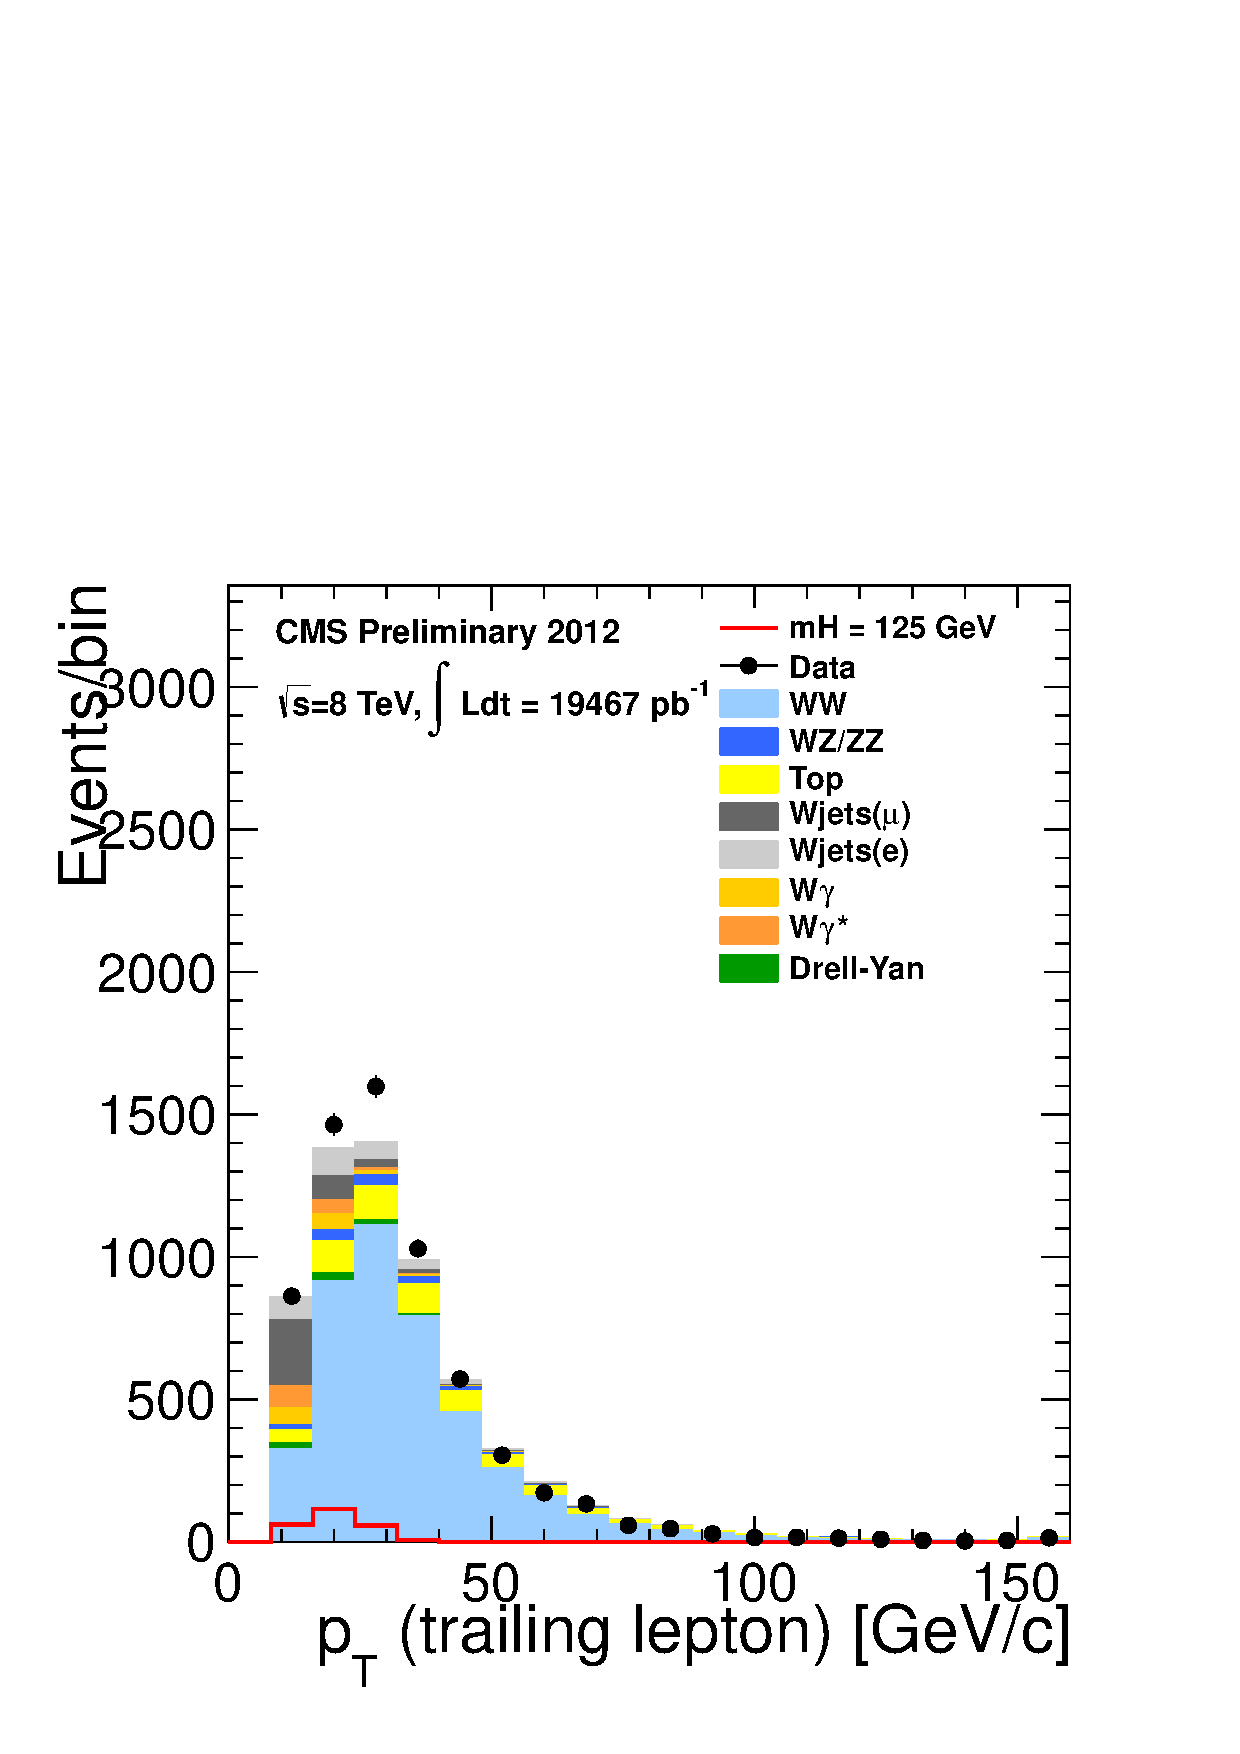
\includegraphics[width=.4\textwidth]{figures/hww_analysis16_0_ALL_of_0j_pt2.pdf}
}
\subfigure[1-Jet]{
\centering
\label{subfig:ww_ptmin_1j}
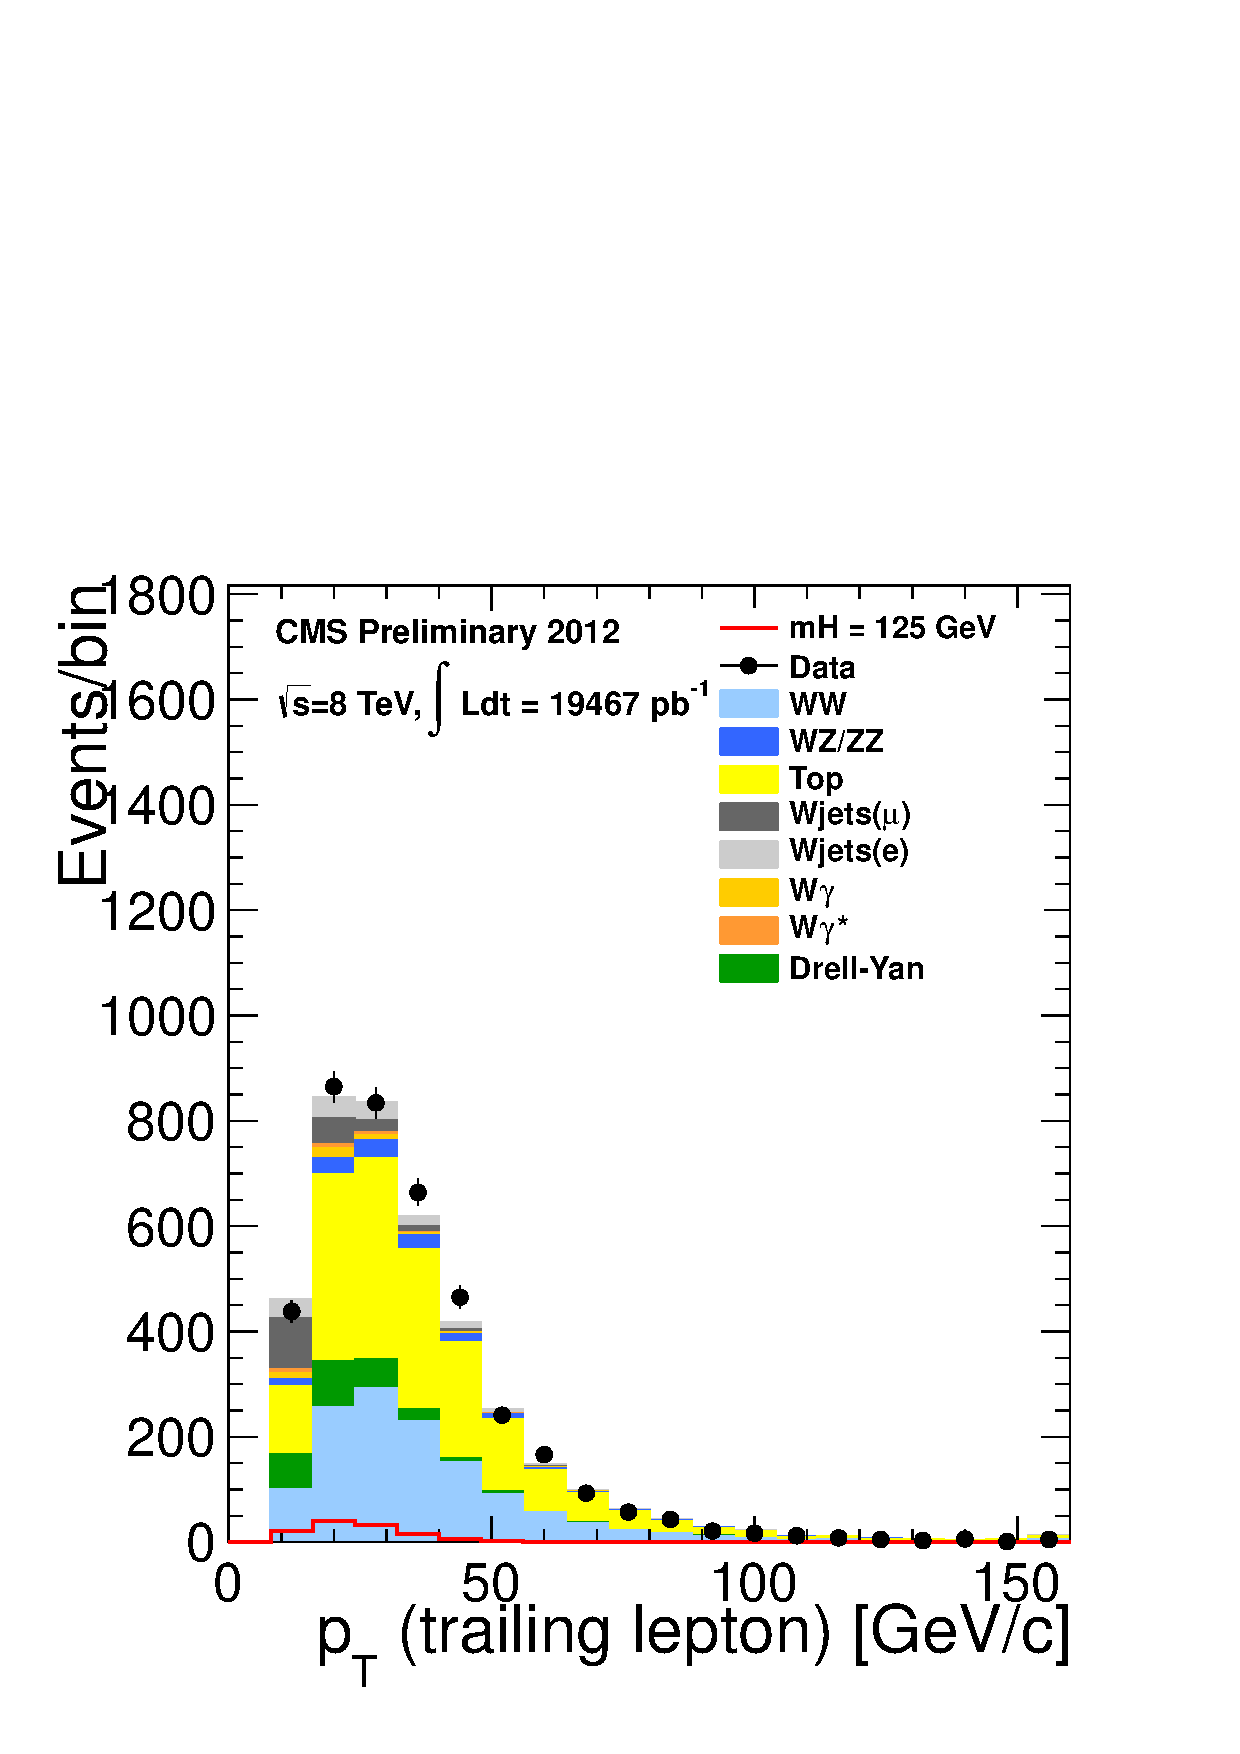
\includegraphics[width=.4\textwidth]{figures/hww_analysis16_0_ALL_of_1j_pt2.pdf}
}\\
\caption{Trailing lepton $p_T$ distribution after WW selection for \intlumiEightTeV of data 
of {\bf DF events} in 0-jet \subref{subfig:ww_ptmin_0j} 1-jet \subref{subfig:ww_ptmin_1j} bins. 
MC is scaled to data-driven estimates for all processes. 
The signal region is blinded with $m_{\ell\ell}>70$ GeV. }
\label{fig:ww_ptmin}
\end{figure}

\begin{figure}[!hbtp]
\centering
\subfigure[0-Jet]{
\centering
\label{subfig:ww_ptmax_0j}
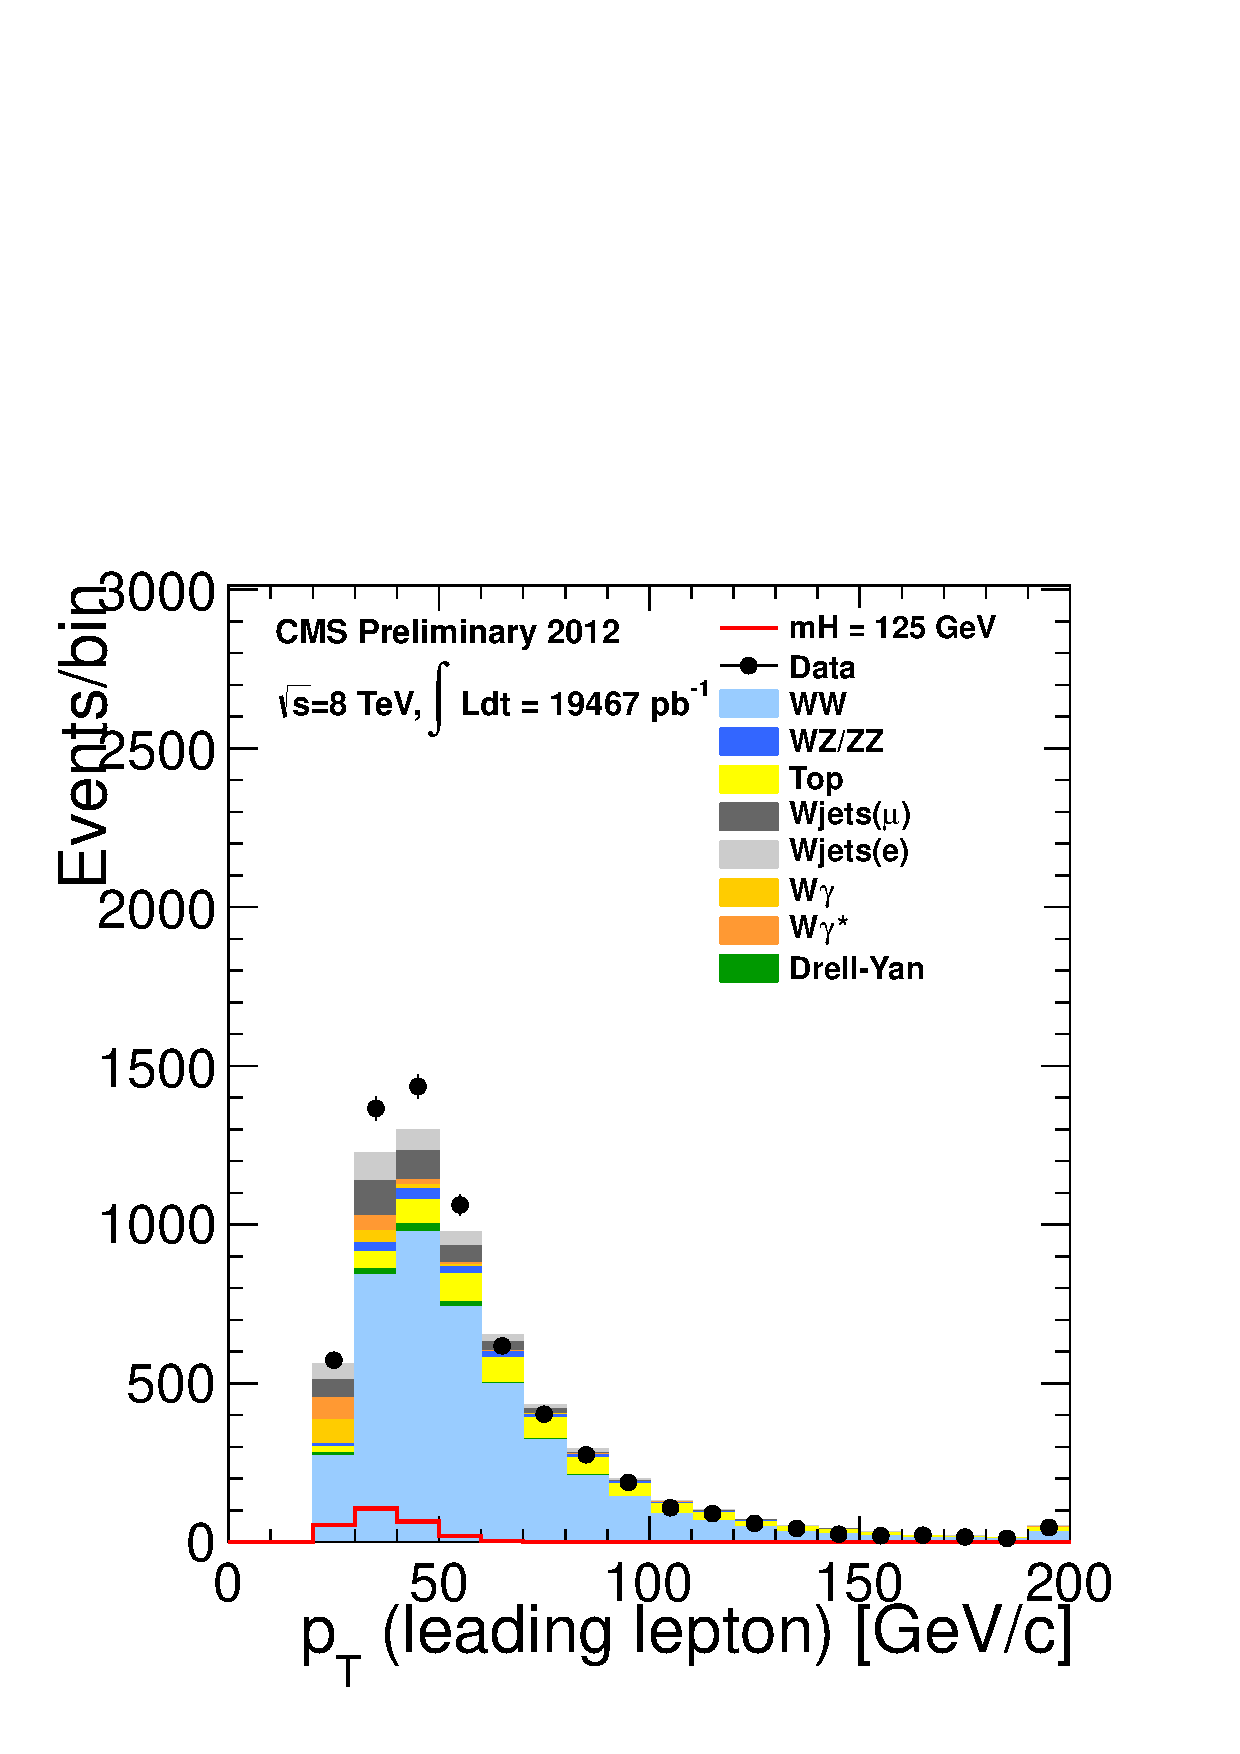
\includegraphics[width=.4\textwidth]{figures/hww_analysis16_0_ALL_of_0j_pt1.pdf}
}
\subfigure[1-Jet]{
\centering
\label{subfig:ww_ptmax_1j}
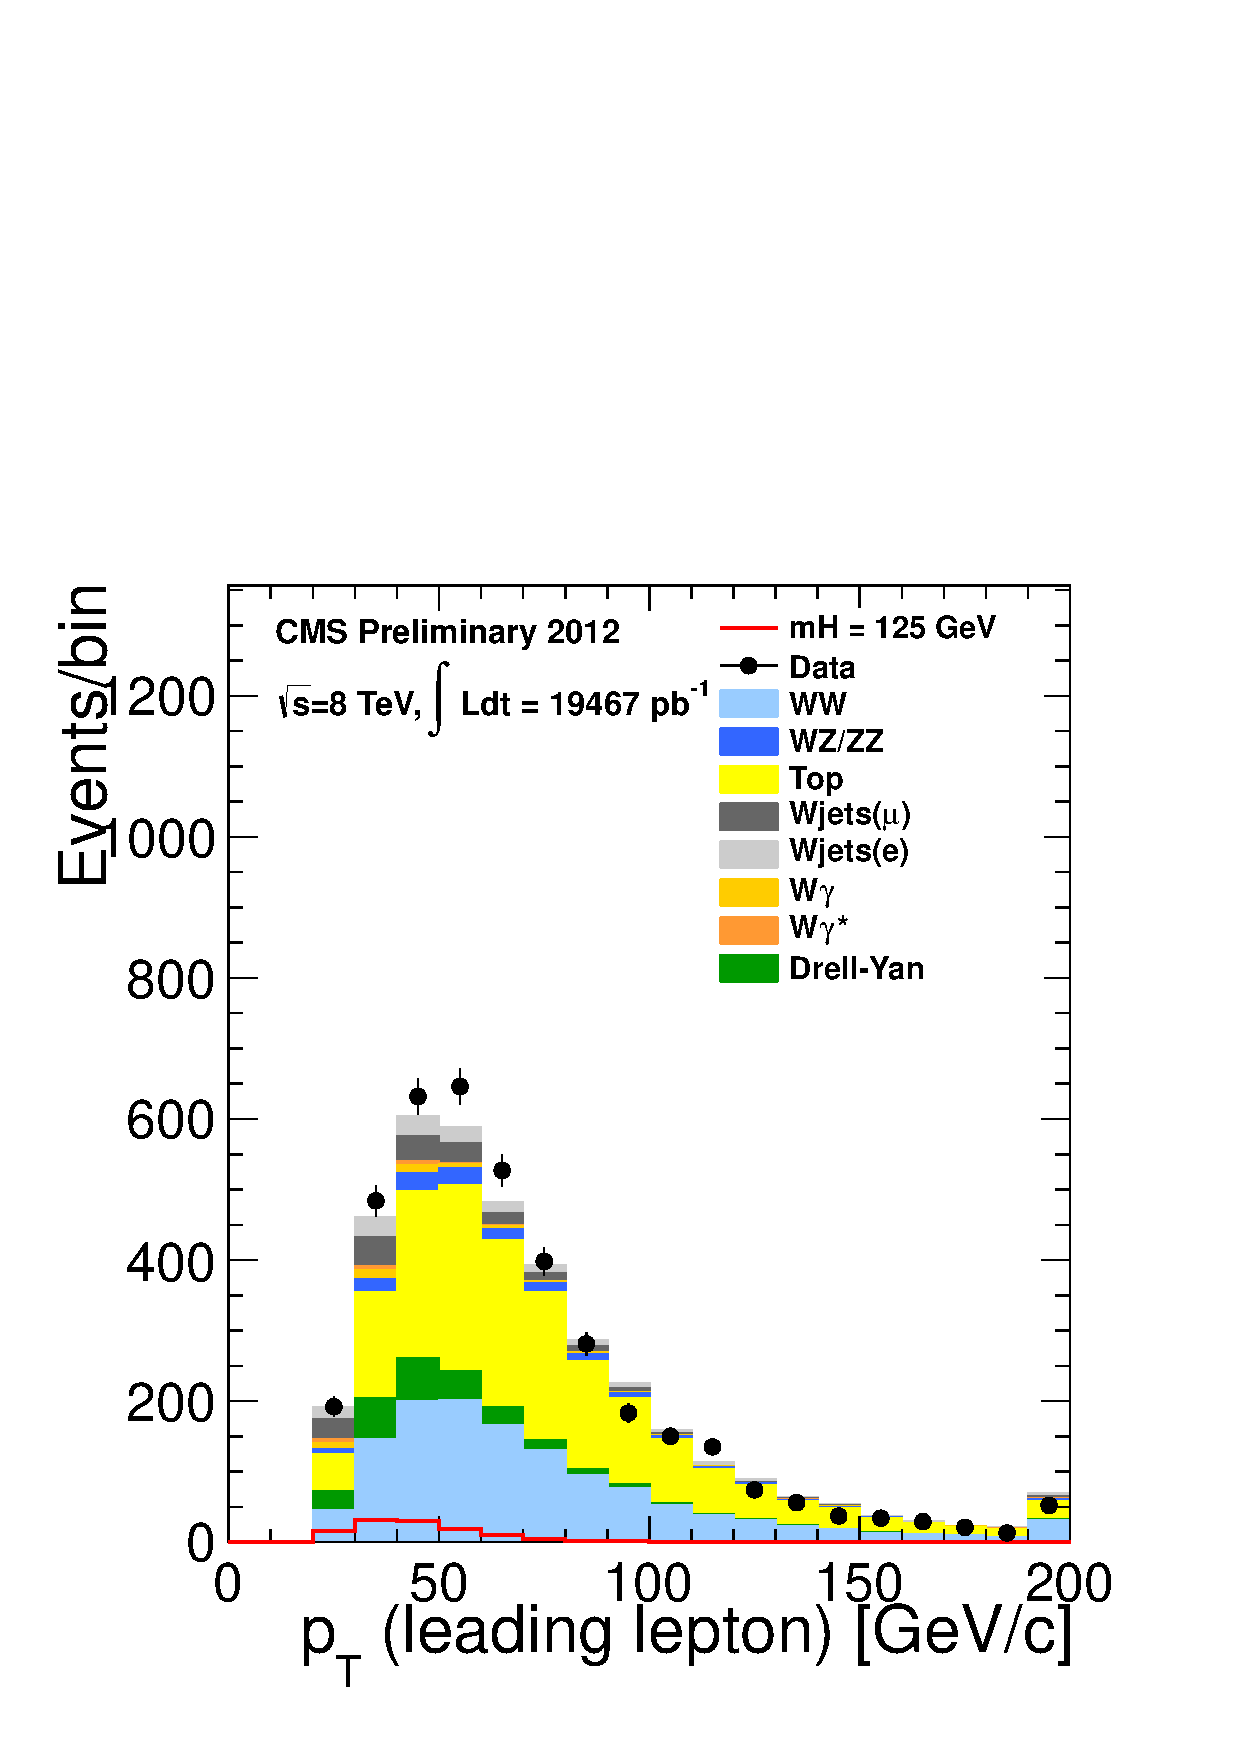
\includegraphics[width=.4\textwidth]{figures/hww_analysis16_0_ALL_of_1j_pt1.pdf}
}\\
\caption{Leading lepton $p_T$ distribution after WW selection for \intlumiEightTeV of data 
of {\bf DF events} in 0-jet \subref{subfig:ww_ptmax_0j} 1-jet \subref{subfig:ww_ptmax_1j} bins.  
MC is scaled to data-driven estimates for all processes.
The signal region is blinded with $m_{\ell\ell}>70$ GeV. }
\label{fig:ww_ptmax}
\end{figure}

\begin{figure}[!hbtp]
\centering
\subfigure[0-Jet]{
\centering
\label{subfig:ww_pmet_0j}
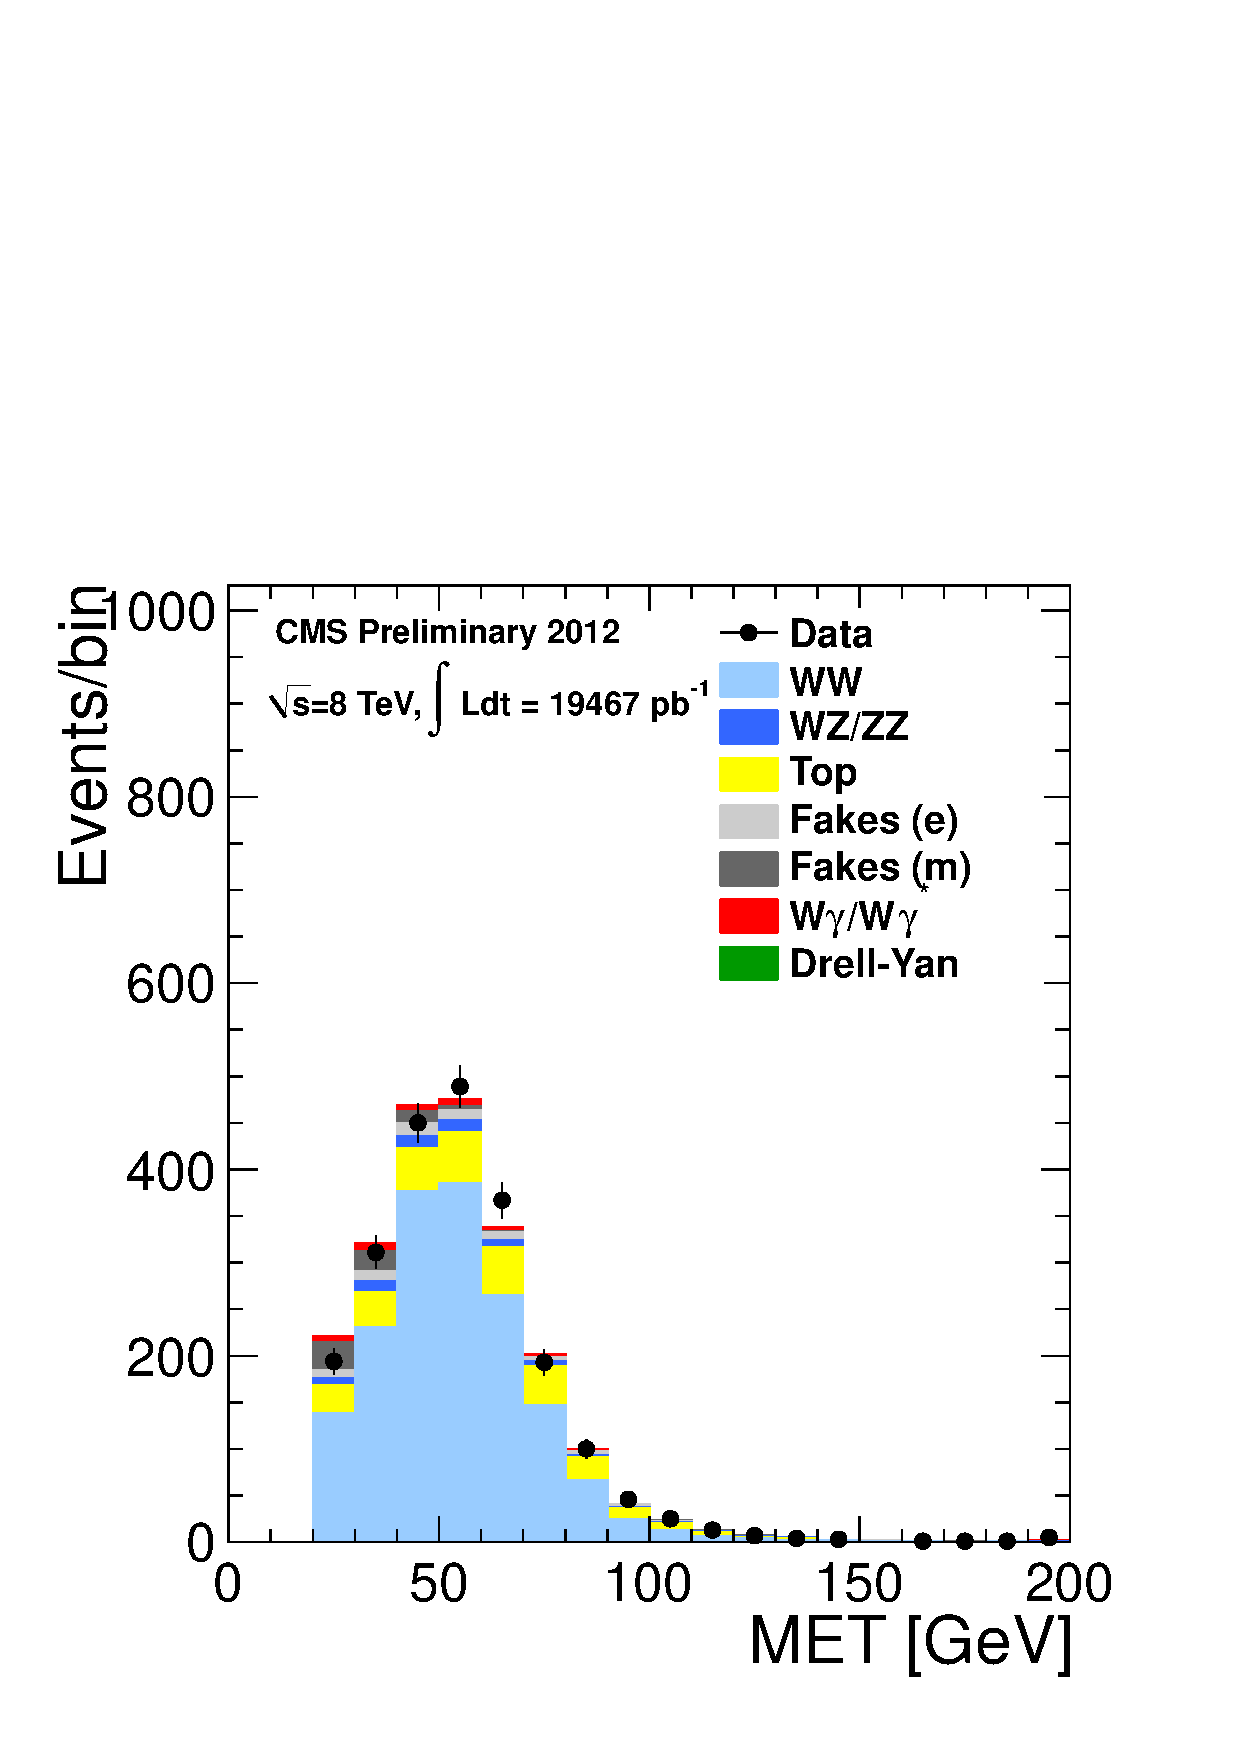
\includegraphics[width=.4\textwidth]{figures/hww_analysis16_0_ALL_of_0j_met.pdf}
}
\subfigure[1-Jet]{
\centering
\label{subfig:ww_pmet_1j}
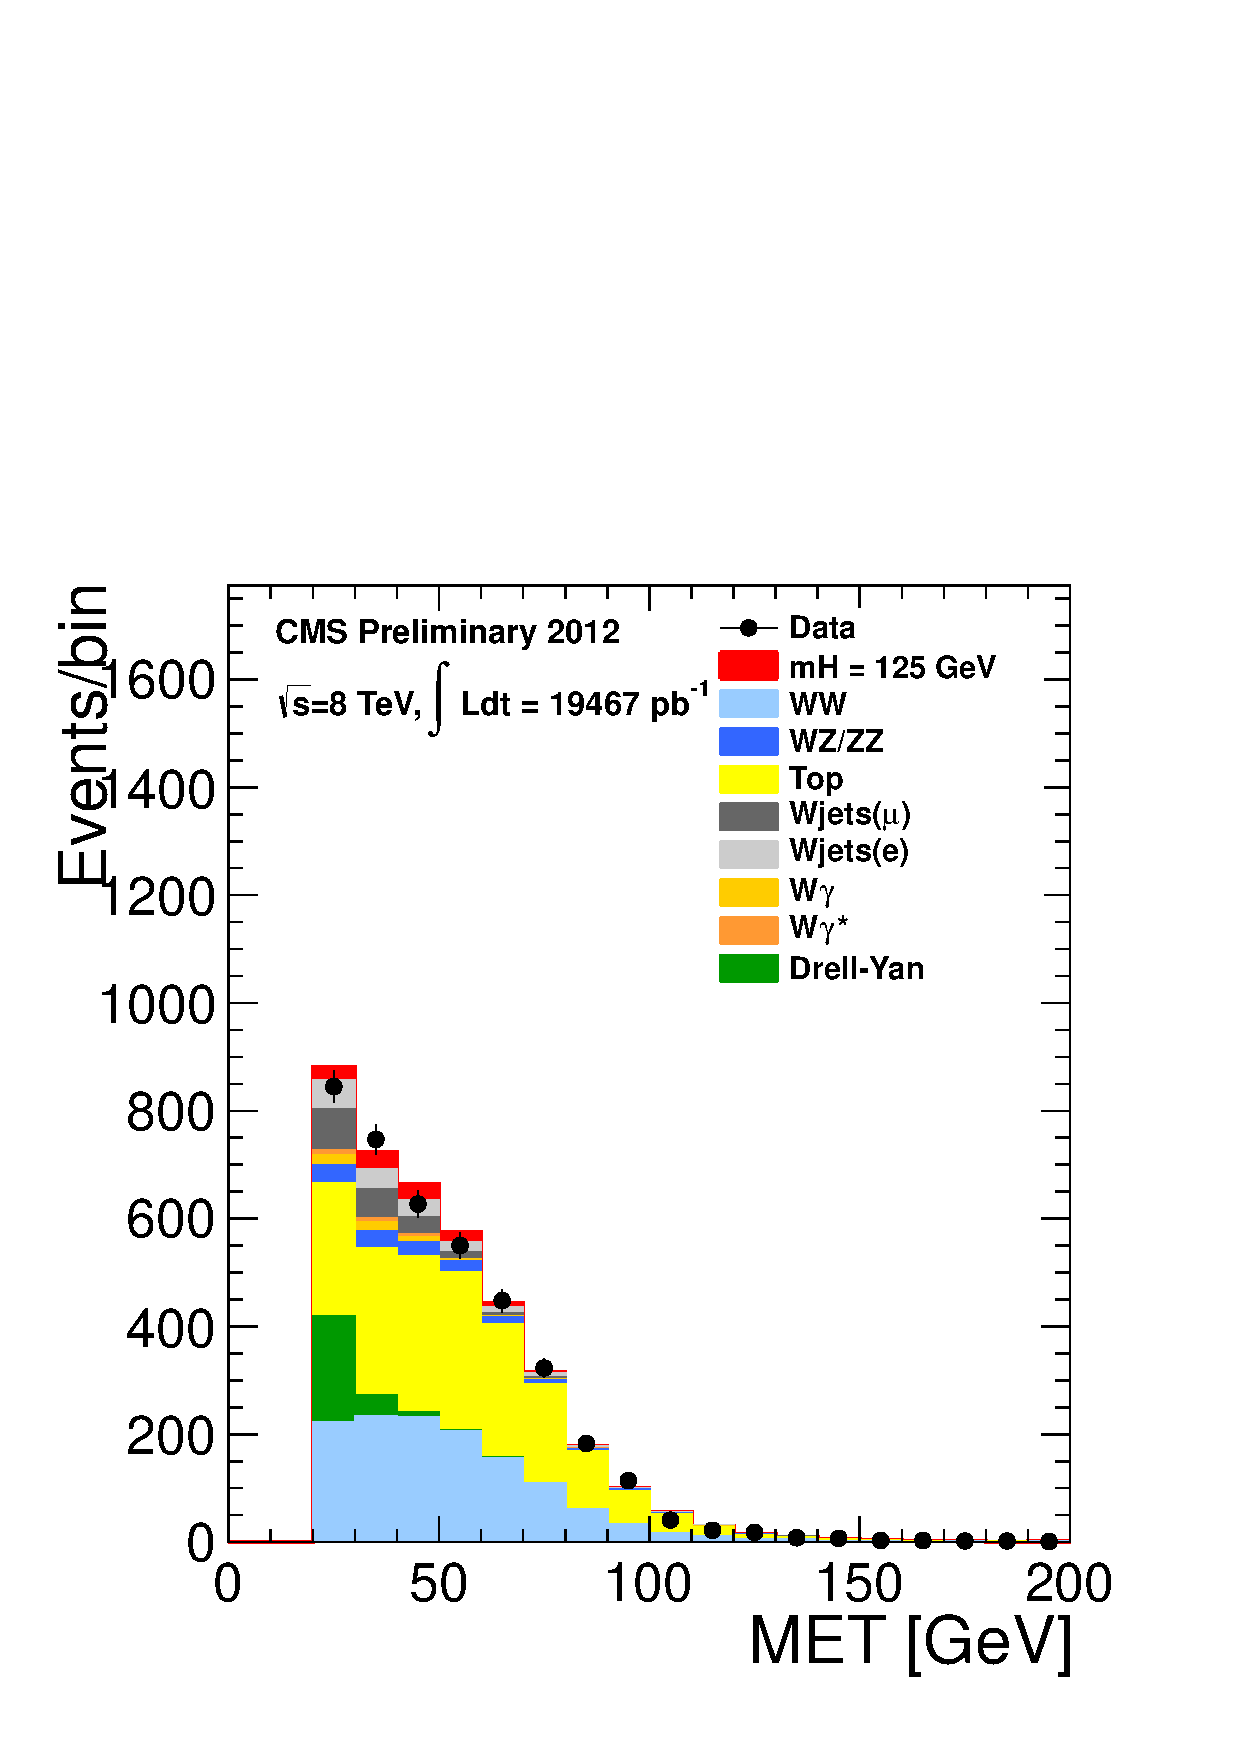
\includegraphics[width=.4\textwidth]{figures/hww_analysis16_0_ALL_of_1j_met.pdf}
}\\
\caption{The $\met$ distributions distribution after WW selection for \intlumiEightTeV of data 
of {\bf DF events} in 0-jet \subref{subfig:ww_pmet_0j} 1-jet \subref{subfig:ww_pmet_1j} bins.   
The MET variable plotted is $min(\text{proj}_\text{trk-MET}, \text{proj}_\text{PFMET})$. 
 MC is scaled to data-driven estimates for all processes.
The signal region is blinded with $m_{\ell\ell}>70$ GeV. }
\label{fig:ww_pmet}
\end{figure}

\begin{figure}[!hbtp]
\centering
\subfigure[0-Jet]{
\centering
\label{subfig:ww_mt_0j}
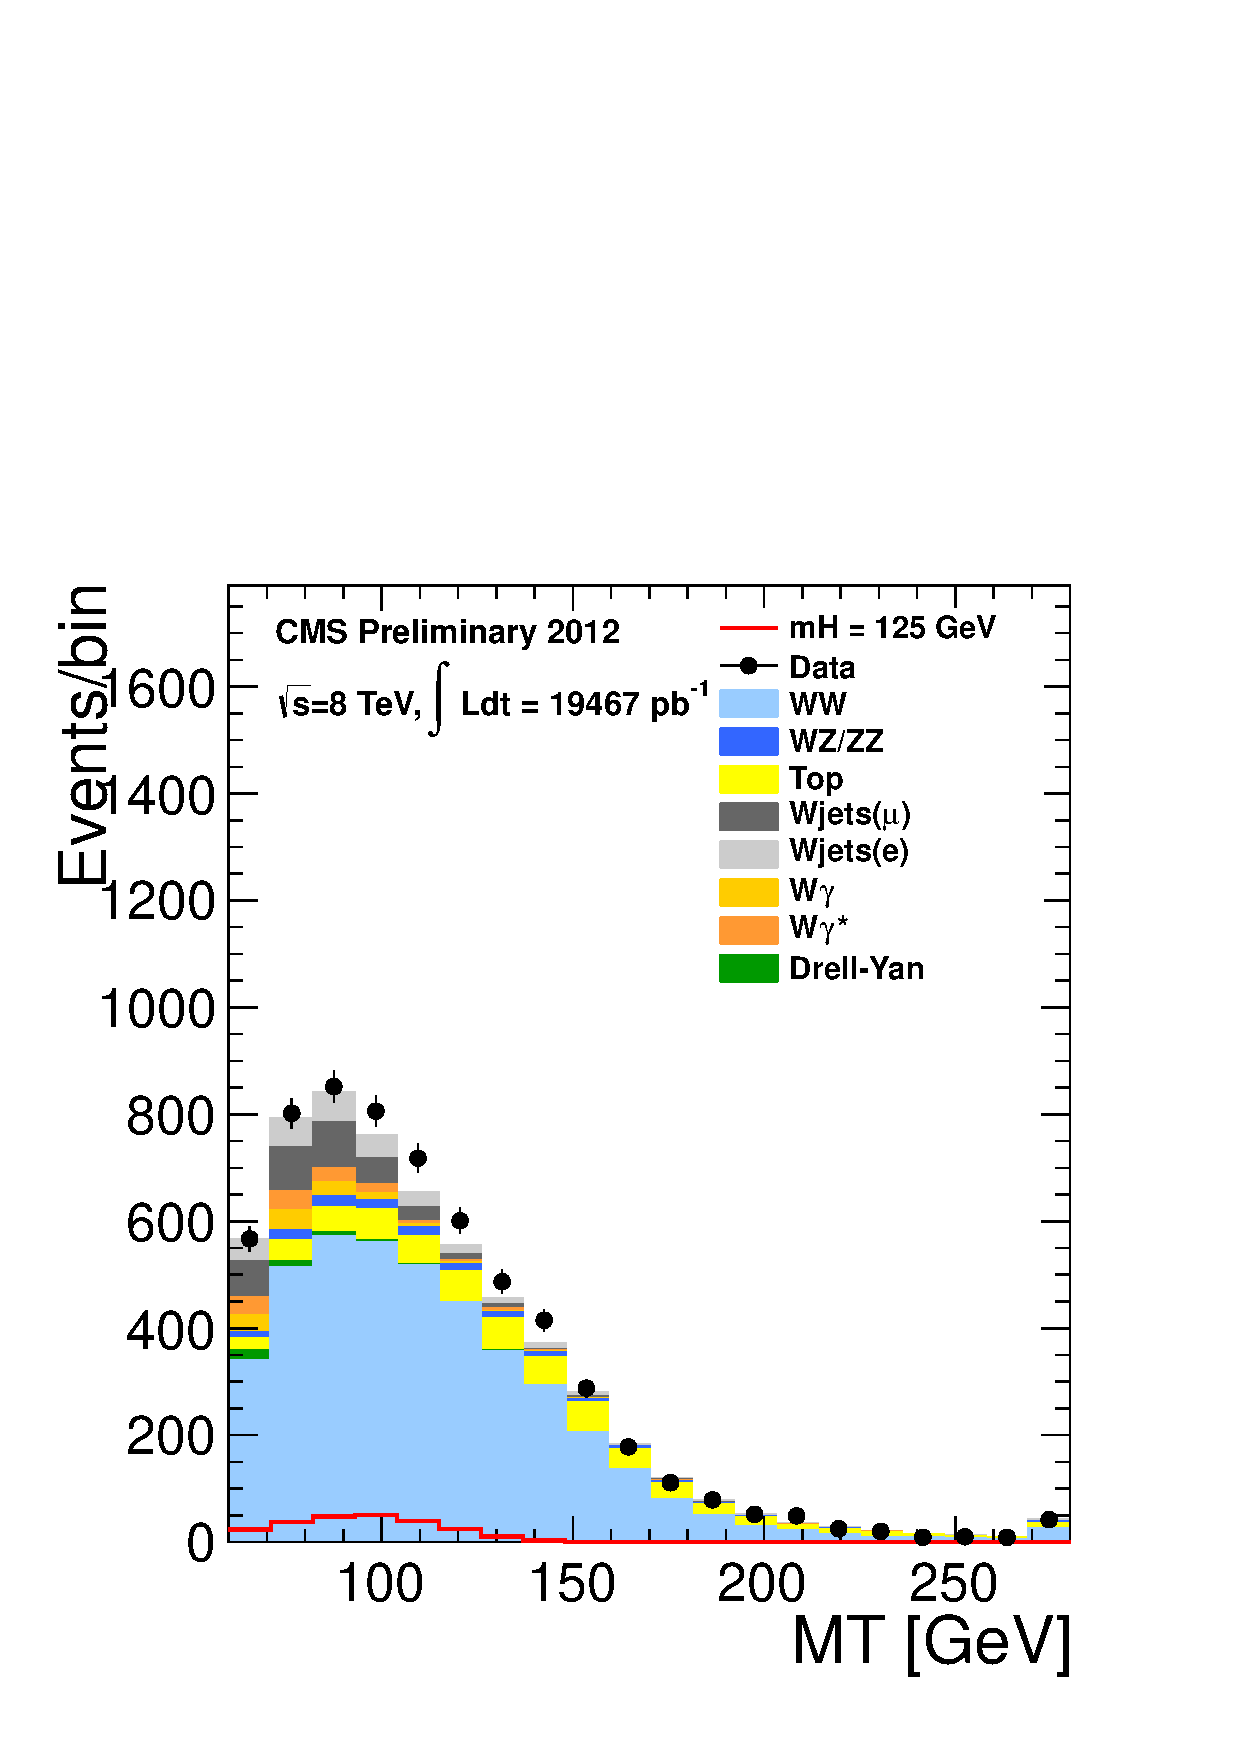
\includegraphics[width=.4\textwidth]{figures/hww_analysis16_0_ALL_of_0j_mt.pdf}
}
\subfigure[1-Jet]{
\centering
\label{subfig:ww_mt_1j}
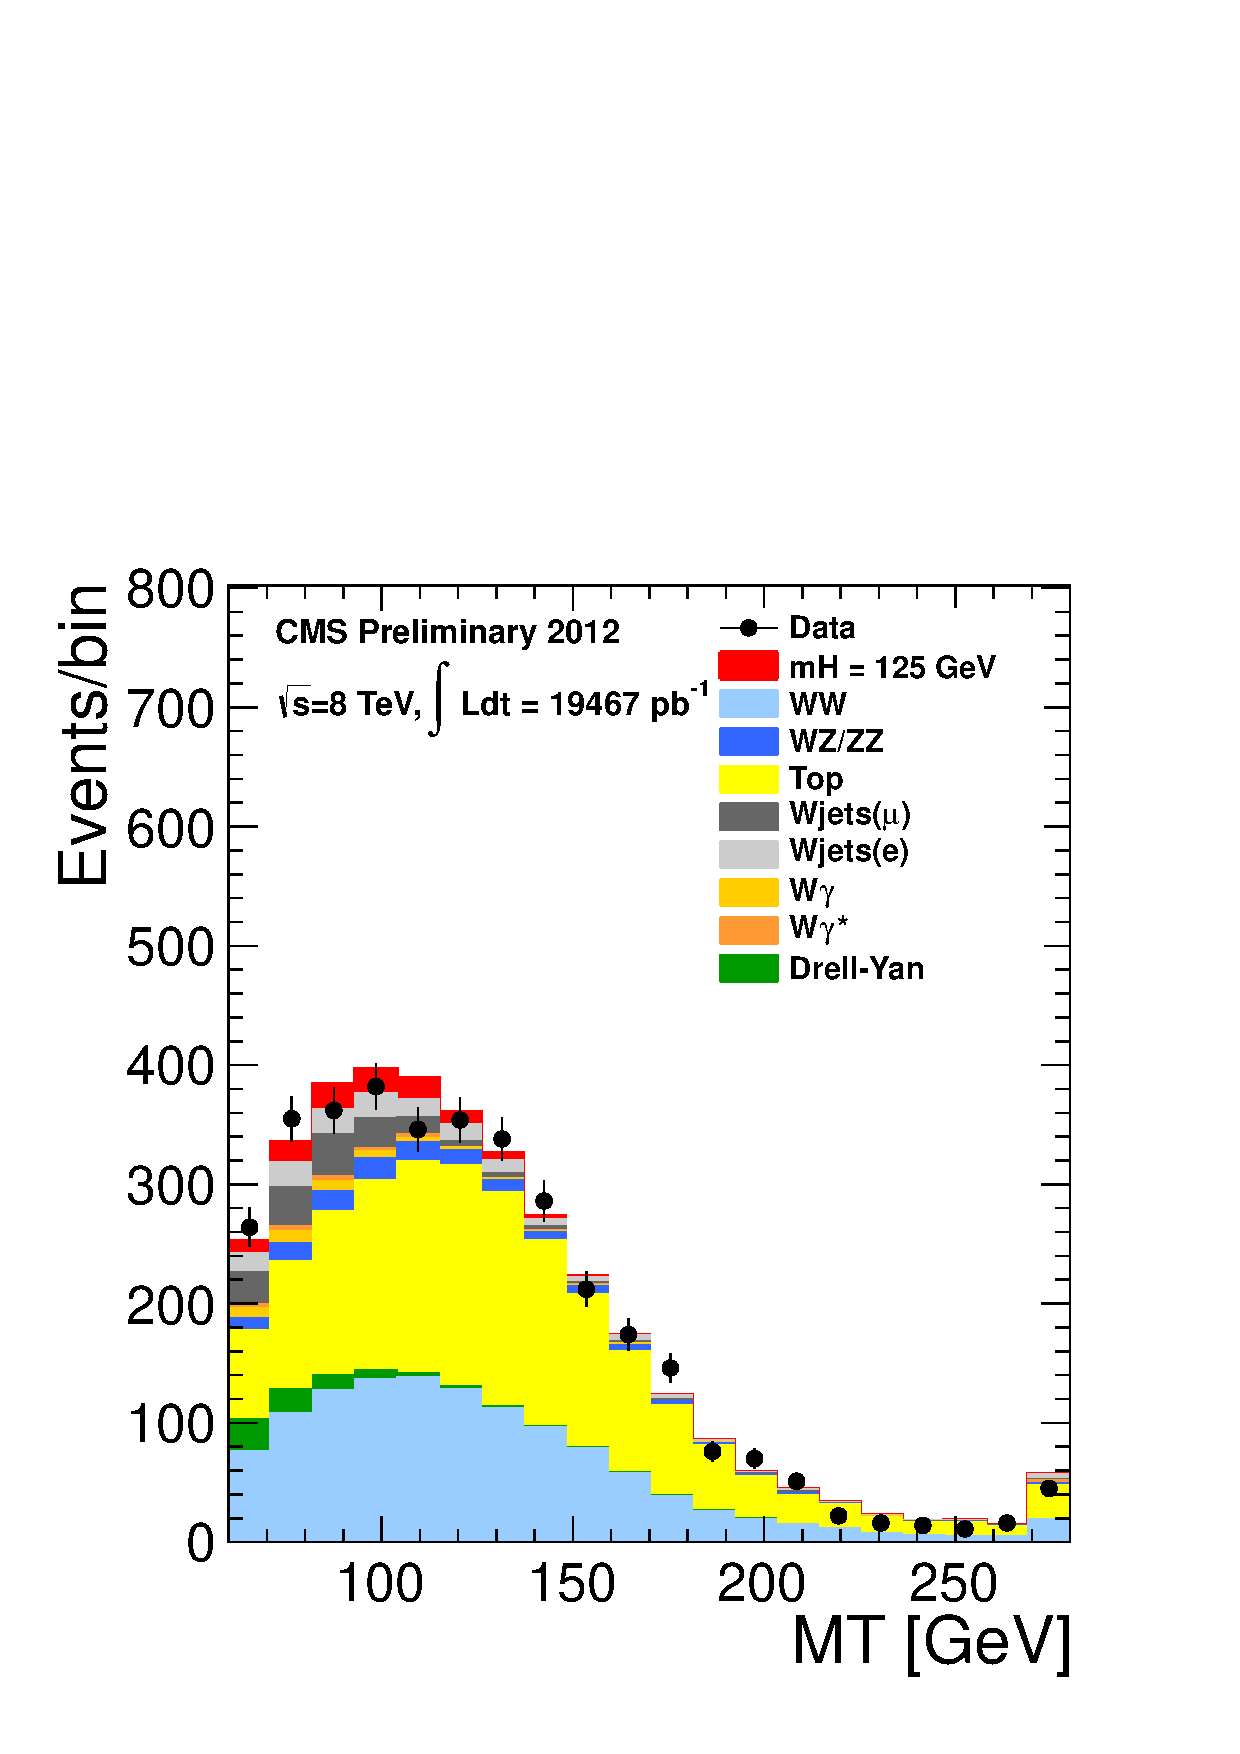
\includegraphics[width=.4\textwidth]{figures/hww_analysis16_0_ALL_of_1j_mt.pdf}
} \\
\caption{Transverse mass distribution after WW selection for \intlumiEightTeV of data 
of {\bf DF events} in 0-jet \subref{subfig:ww_mt_0j} 1-jet \subref{subfig:ww_mt_1j} bins.   
MC is scaled to data-driven estimates for all processes.
The signal region is blinded with $m_{\ell\ell}>70$ GeV. }
\label{fig:ww_mt}
\end{figure}

\begin{figure}[!hbtp]
\centering
\subfigure[0-Jet]{
\centering
\label{subfig:ww_dilmass_0j}
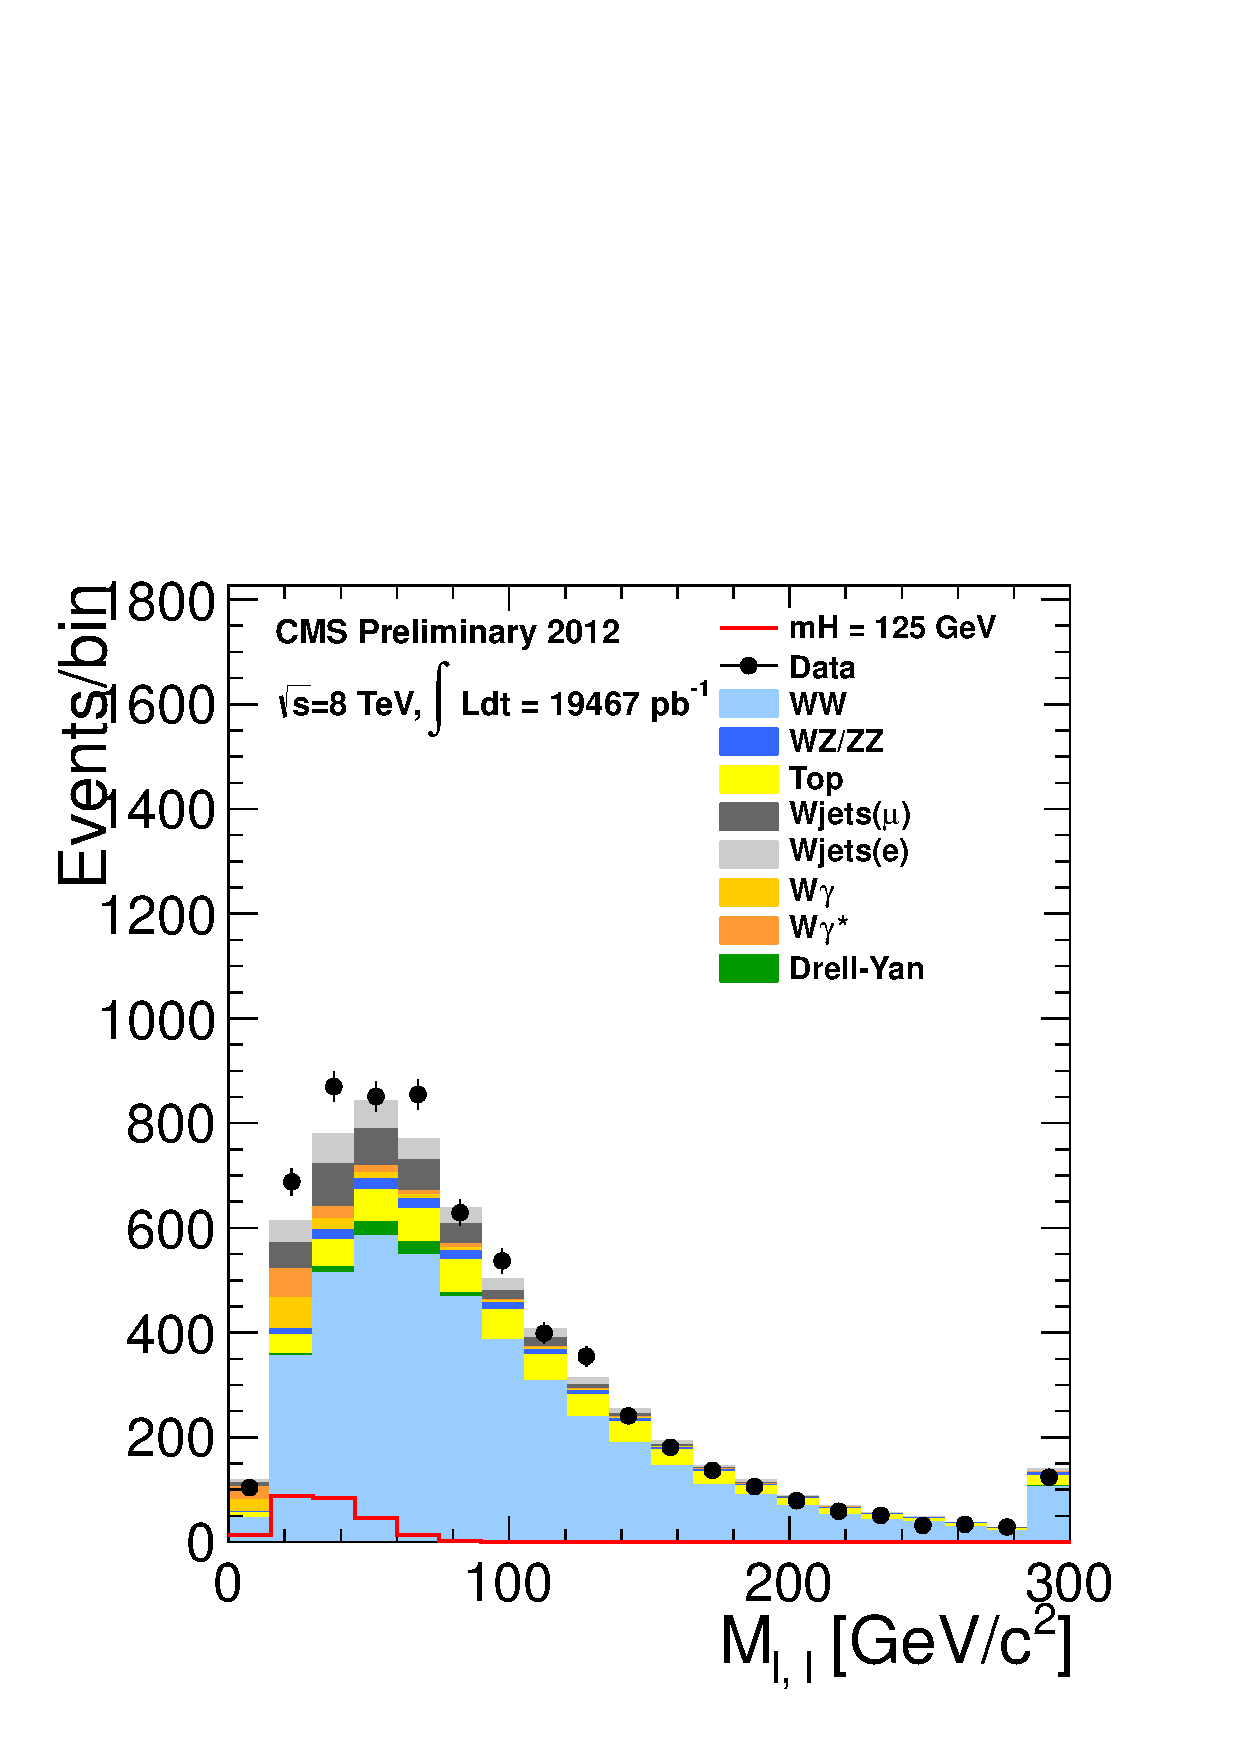
\includegraphics[width=.4\textwidth]{figures/hww_analysis16_0_ALL_of_0j_mll.pdf}
}
\subfigure[1-Jet]{
\centering
\label{subfig:ww_dilmass_1j}
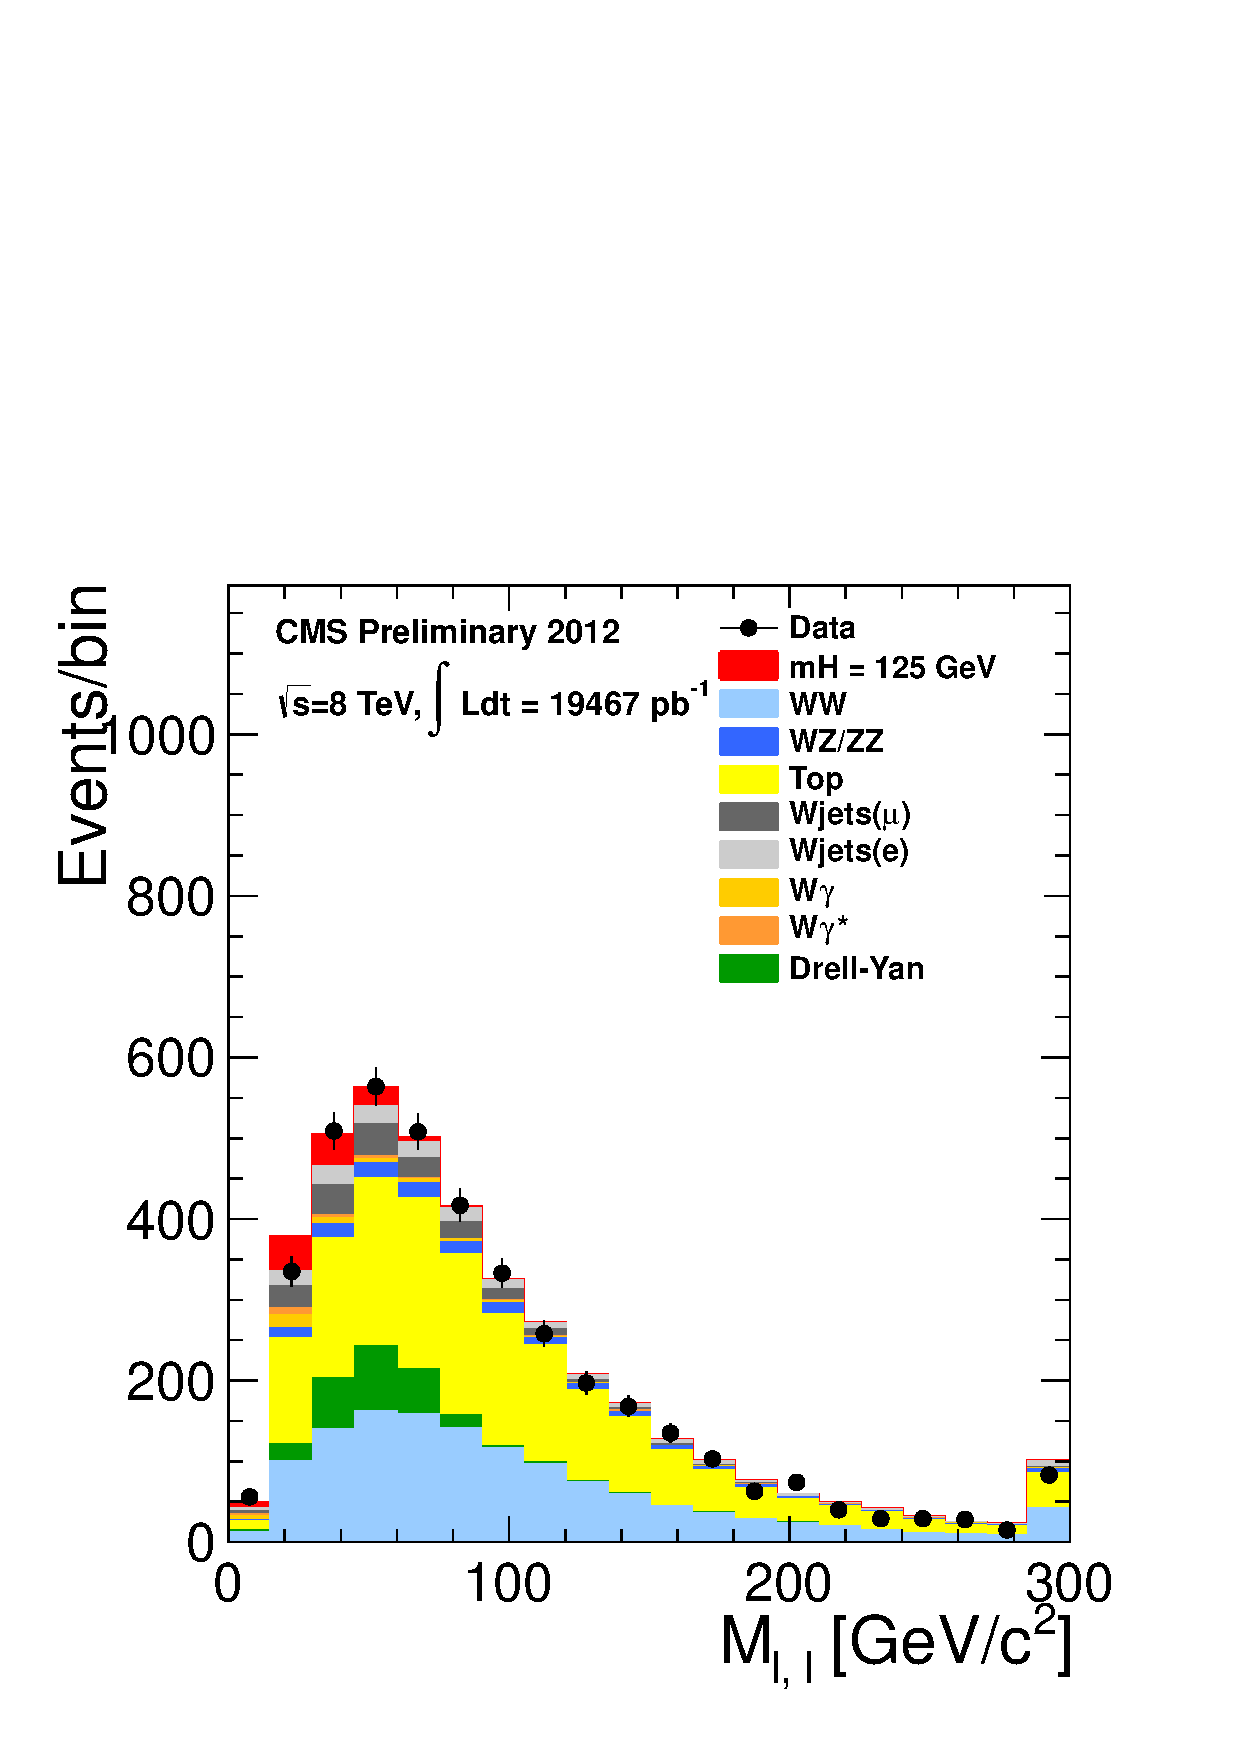
\includegraphics[width=.4\textwidth]{figures/hww_analysis16_0_ALL_of_1j_mll.pdf}
} \\
\caption{Invariant dilepton mass distribution after WW selection for \intlumiEightTeV of data  
of {\bf DF events} in 0-jet \subref{subfig:ww_dilmass_0j} 1-jet \subref{subfig:ww_dilmass_1j} bins.   
MC is scaled to data-driven estimates for all processes.
The signal region is blinded with $m_{\ell\ell}>70$ GeV. }
\label{fig:ww_dilmass}
\end{figure}

\begin{figure}[!hbtp]
\centering
\subfigure[0-Jet]{
\centering
\label{subfig:ww_deltaphi_0j}
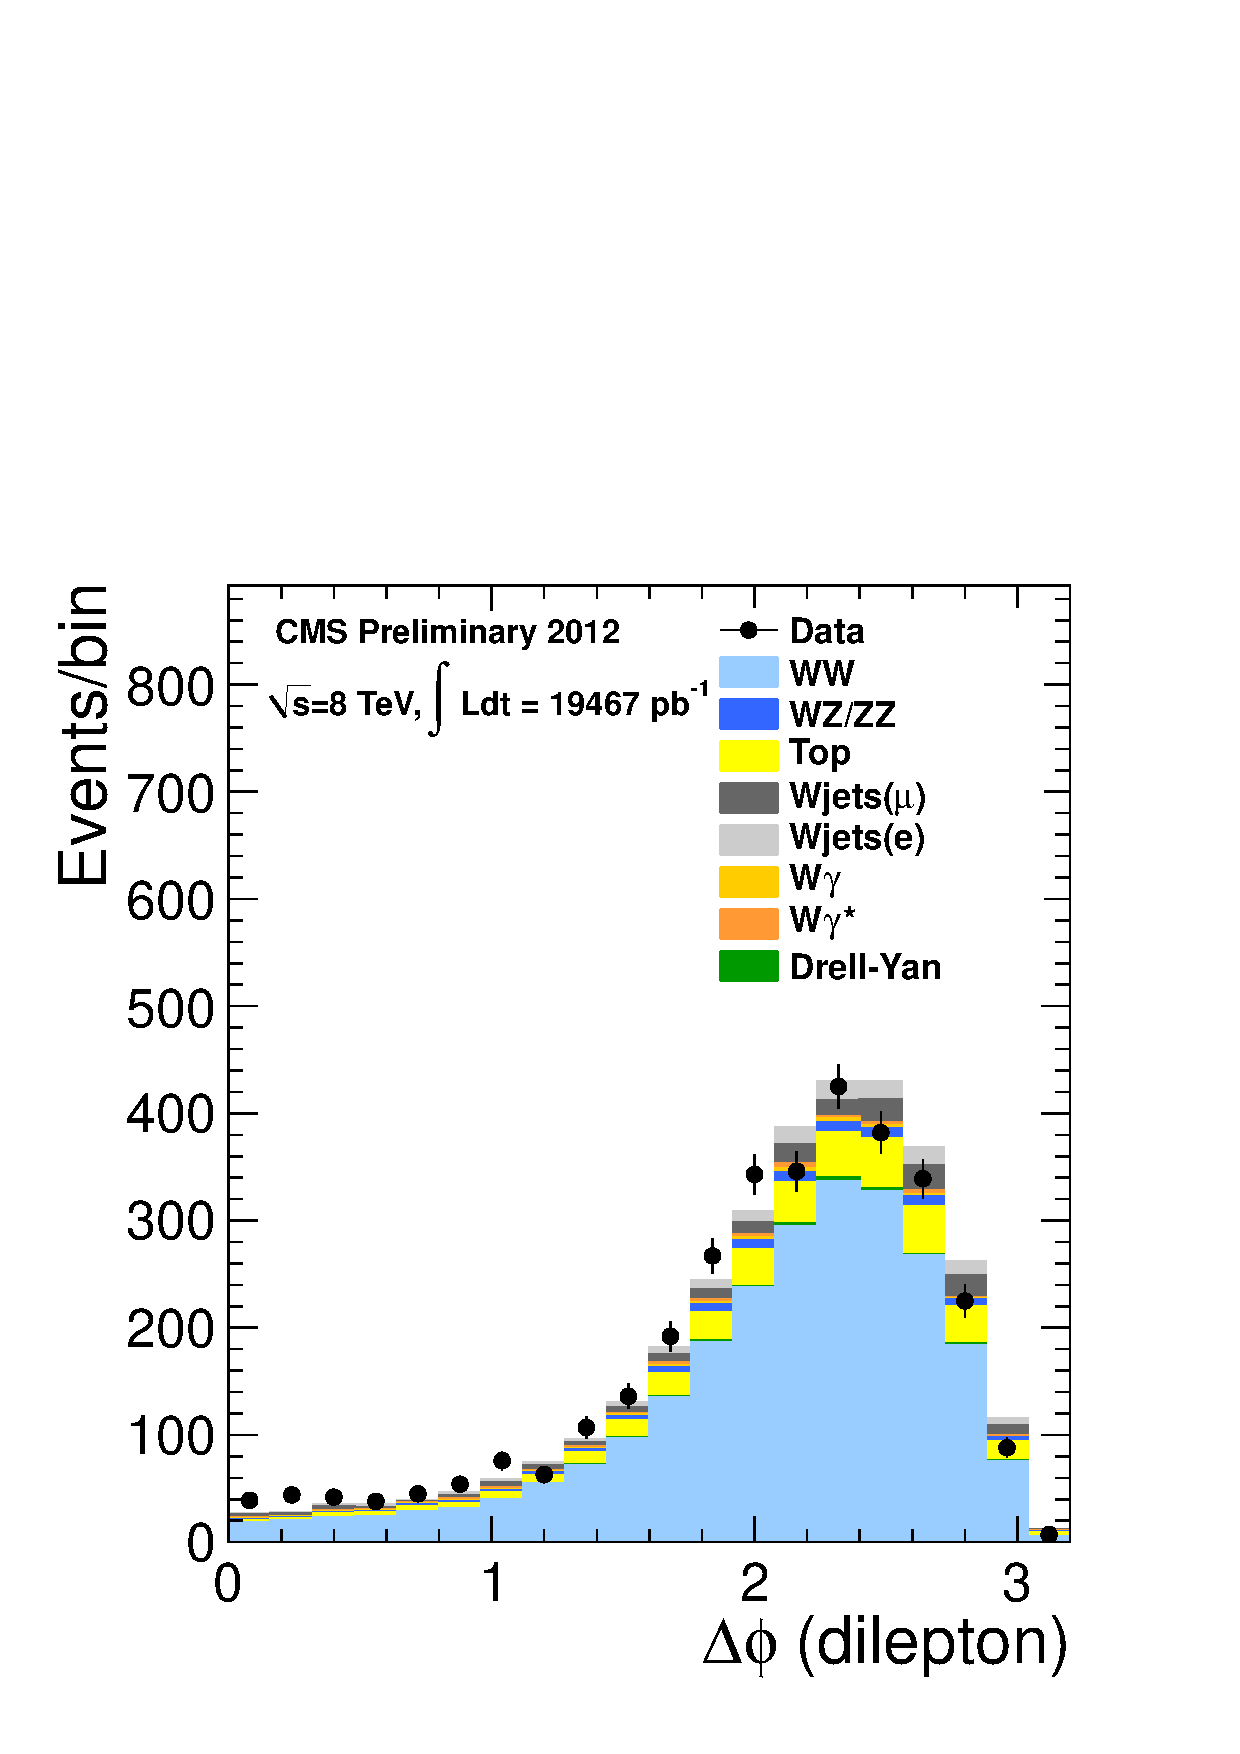
\includegraphics[width=.4\textwidth]{figures/hww_analysis16_0_ALL_of_0j_dphi.pdf}
}
\subfigure[1-Jet]{
\centering
\label{subfig:ww_deltaphi_1j}
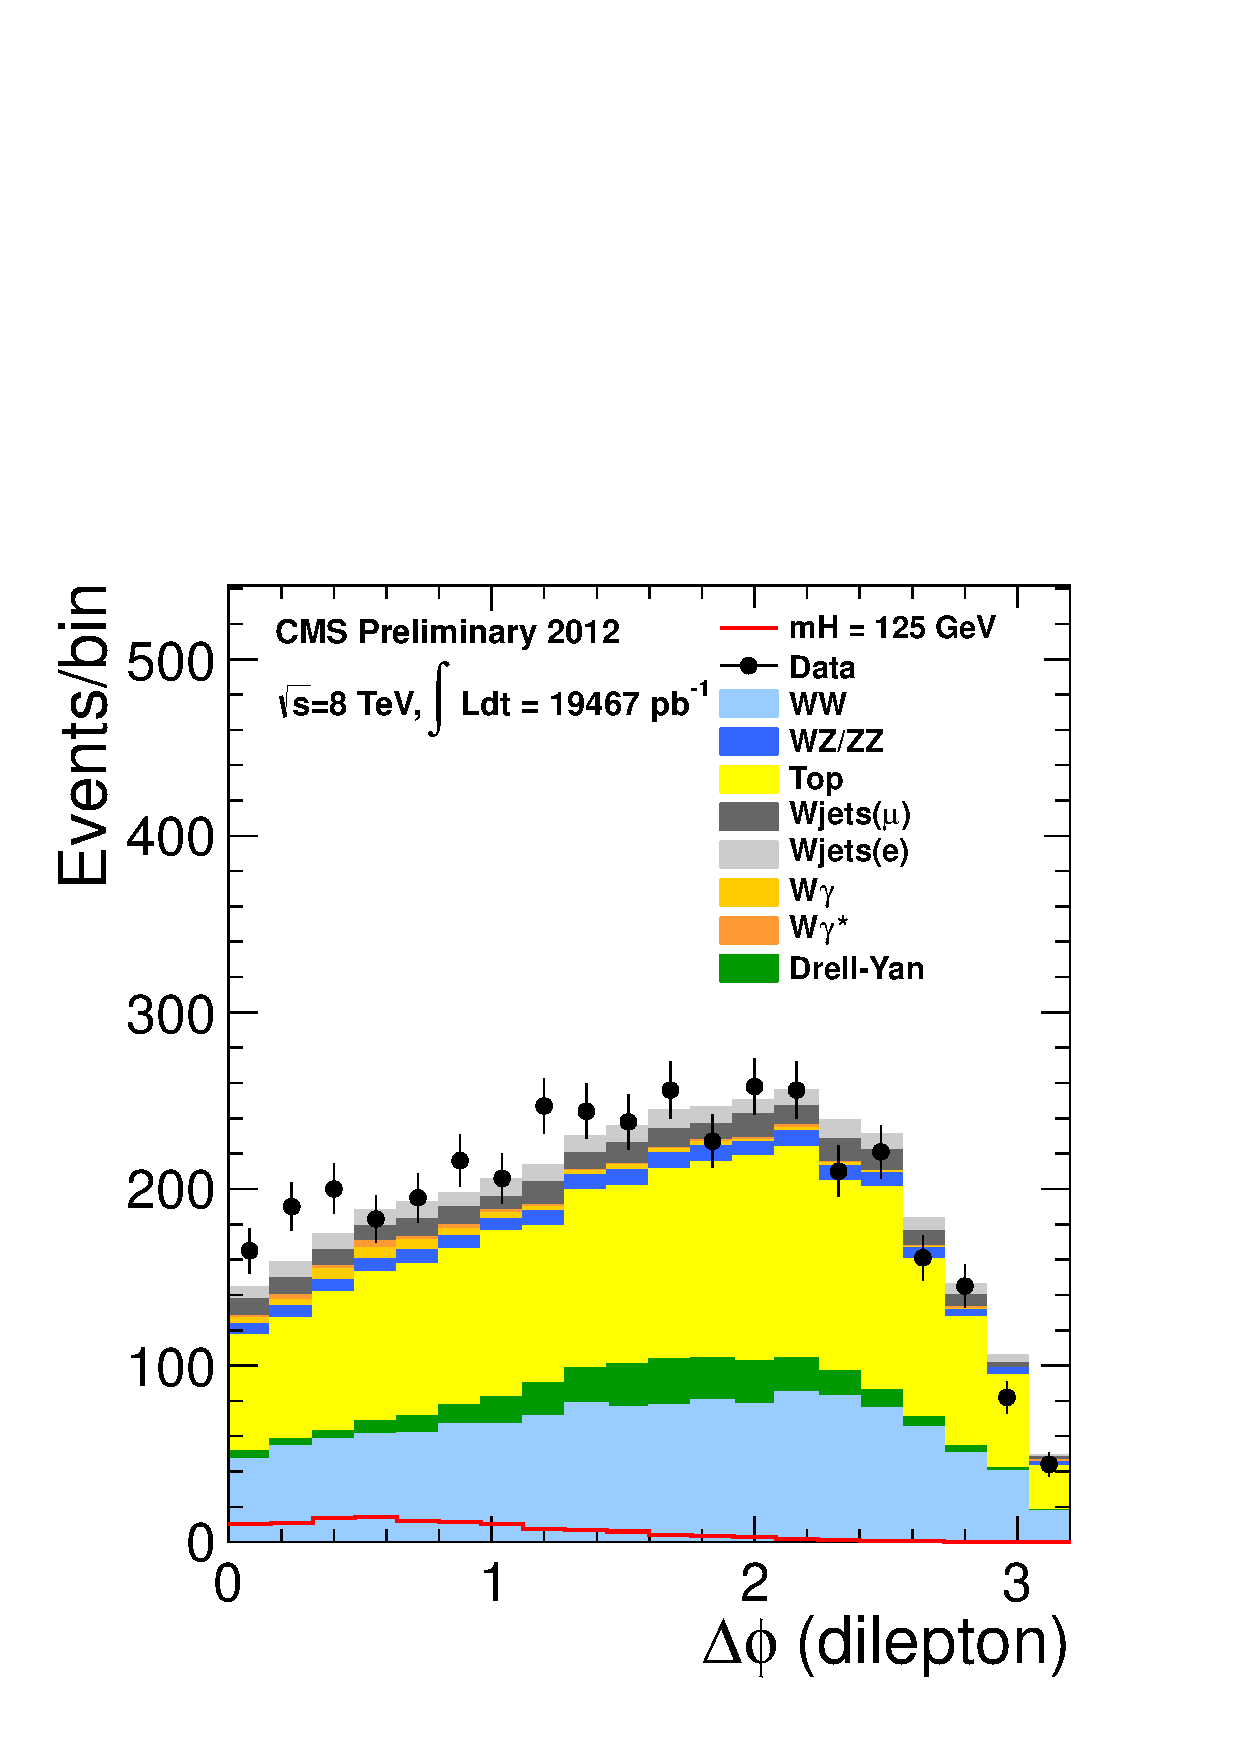
\includegraphics[width=.4\textwidth]{figures/hww_analysis16_0_ALL_of_1j_dphi.pdf}
} \\
\caption{Dilepton $\Delta\phi$ distribution after WW selection for \intlumiEightTeV of data 
of {\bf DF events} in 0-jet \subref{subfig:ww_deltaphi_0j} 1-jet \subref{subfig:ww_deltaphi_1j} bins.   
MC is scaled to data-driven estimates.
The signal region is blinded with $m_{\ell\ell}>70$ GeV. }
\label{fig:ww_deltaphi}
\end{figure}

%%%%%%%%%%%%%%%%%%%%%%%%%%%%%%%%%%%%%%%%%%%%%%%%%%%%%%%%%%% 
\begin{table}[ht!]
\begin{center}
\begin{tabular}{c | c | c } 
\hline
            & \multicolumn{1}{c|}{0-jet} & \multicolumn{1}{c}{1-jet} \\
mass [\GeV] & scale factor & scale factor \\
\hline
            \multicolumn{3}{c}{Cut-based} \\
\hline
115 &  1.09  $\pm$  0.06  &  0.93  $\pm$  0.10 \\
120 &  1.09  $\pm$  0.06  &  0.93  $\pm$  0.10 \\
125 &  1.09  $\pm$  0.06  &  0.93  $\pm$  0.10 \\
130 &  1.09  $\pm$  0.06  &  0.93  $\pm$  0.10 \\
135 &  1.09  $\pm$  0.06  &  0.93  $\pm$  0.10 \\
140 &  1.09  $\pm$  0.06  &  0.94  $\pm$  0.09 \\
150 &  1.08  $\pm$  0.06  &  0.94  $\pm$  0.10 \\
160 &  1.08  $\pm$  0.06  &  0.94  $\pm$  0.10 \\
170 &  1.07  $\pm$  0.06  &  0.94  $\pm$  0.10 \\
180 &  1.07  $\pm$  0.06  &  0.94  $\pm$  0.10 \\
190 &  1.06  $\pm$  0.06  &  0.93  $\pm$  0.10 \\
200 &  1.07  $\pm$  0.06  &  0.93  $\pm$  0.10 \\
\hline \hline
            \multicolumn{3}{c}{Shape} \\
\hline
All masses & 1.16  $\pm$  0.06  &  1.04  $\pm$  0.10 \\ 
\hline
\end{tabular}
\caption{WW background estimation for cut-based and shape analyses.}
\label{tab:ww_est}
\end{center}
\end{table}

%%%%%%%%%%%%%%%%%%%%%%%%%%%%%%

\clearpage
\subsection{Final Results for the Higgs Search with \intlumiEightTeV{}}
\label{sec:search_results}

\textcolor{red}{NUMBER NOT UPDATED YET} 

Here we present three sets of results based on events with
different lepton flavor. 

The expected and observed upper limits at 95\% C.L.
for the cut-based shape analysis in all categories are shown in Table~\ref{tab:ulscut}.
The corresponding limits when the 2D analysis is used 
in the DF 0 and 1-jet categories is shown in Table~\ref{tab:uls_2d01_cut2_cutsf}.
The results are shown in Figures~\ref{fig:ulscut} 
and~\ref{fig:uls_2d01_cut2_cutsf}, respectively.
In both analyses, the VBF category is analysed using the cut based approach.

%The expected and observed upper limits at 95\% C.L. for the cut based and
%multivariate analyses are shown in Tables~\ref{tab:cutbase_uls}
%and~\ref{tab:mvabase_uls}, respectively. The corresponding exclusion
%limits are shown in Figure~\ref{fig:uls}. The detailed event yields 
%for both analyses are summarized in Appendices.~\ref{app:appendix_cutresults} 
%and~\ref{app:appendix_bdtresults}. 
The expected and observed upper limits at 95\% C.L. for the individual channels 
are summarized in Appendix~\ref{app:appendix_limits_bychannel}. 
%The results of the shape analysis using the dilepton mass single variable are 
%summarized in Appendix~\ref{app:appendix_mll_bdt2011}.
%The results of the shape analysis based on the Matrix Element method 
%are summarized in Appendix~\ref{app:appendix_me}. 
We also calculate the expected and observed significance.
Results are summarized in Table~\ref{tab:significance_8TeV}.


%%%%%%%%%%%%%%%%%
% plot
\begin{figure}[!hbtp]
\centering
%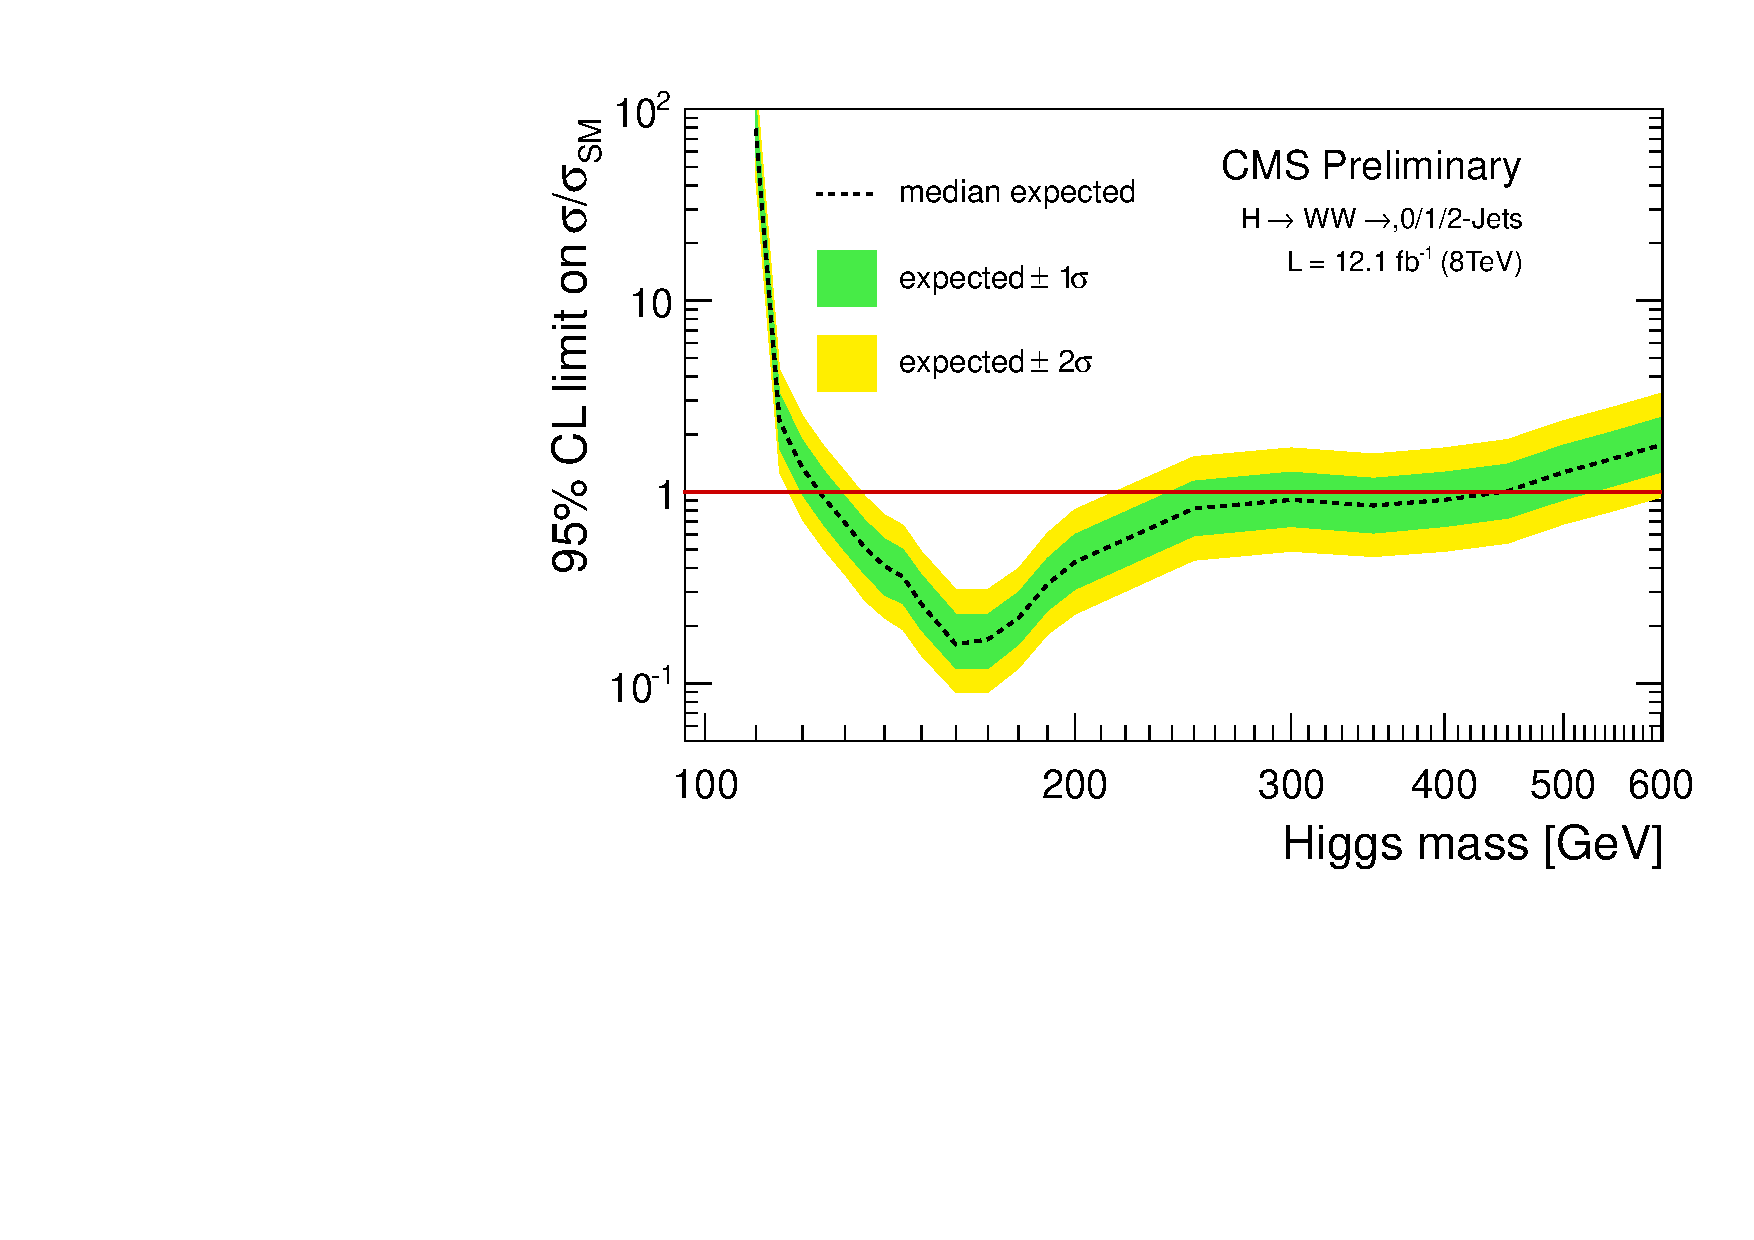
\includegraphics[width=.75\textwidth]{figures/table_limits_nj_cut_log.pdf}
\caption{Expected upper limits for SM Higgs in $\intlumiEightTeV$ at 8 TeV in all final states combined.
Cut-based result is used. }
\label{fig:ulscut}
\end{figure}
% table
\begin{table}[!htbp]
\begin{center}
\begin{tabular}{c c c c c}
\hline
\vspace{-3mm} && \\
Higgs Mass & Observed  & Median expected & Expected range for 68\% & Expected range for 95\%   \\
\hline
110 & 8.51 & 4.10 & [2.96, 5.71] & [2.20, 7.65] \\
115 & 4.38 & 2.16 & [1.55, 3.00] & [1.16, 4.02] \\
120 & 2.18 & 1.25 & [0.90, 1.74] & [0.67, 2.34] \\
125 & 1.60 & 0.86 & [0.62, 1.20] & [0.46, 1.61] \\
130 & 1.34 & 0.64 & [0.46, 0.89] & [0.34, 1.19] \\
135 & 0.97 & 0.48 & [0.34, 0.66] & [0.26, 0.89] \\
140 & 0.73 & 0.39 & [0.28, 0.54] & [0.21, 0.73] \\
150 & 0.56 & 0.26 & [0.19, 0.36] & [0.14, 0.49] \\
160 & 0.30 & 0.16 & [0.12, 0.23] & [0.09, 0.31] \\
170 & 0.27 & 0.17 & [0.12, 0.23] & [0.09, 0.31] \\
180 & 0.42 & 0.22 & [0.16, 0.30] & [0.12, 0.40] \\
190 & 0.56 & 0.33 & [0.24, 0.45] & [0.18, 0.61] \\
200 & 0.85 & 0.43 & [0.31, 0.60] & [0.23, 0.81] \\
250 & 1.11 & 0.82 & [0.59, 1.13] & [0.44, 1.52] \\
300 & 1.07 & 0.92 & [0.66, 1.27] & [0.49, 1.71] \\
350 & 0.73 & 0.85 & [0.61, 1.18] & [0.46, 1.58] \\
400 & 0.70 & 0.90 & [0.65, 1.26] & [0.49, 1.69] \\
450 & 0.69 & 1.00 & [0.72, 1.39] & [0.53, 1.86] \\
500 & 0.83 & 1.24 & [0.89, 1.73] & [0.67, 2.32] \\
550 & 1.08 & 1.47 & [1.06, 2.04] & [0.79, 2.74] \\
600 & 1.42 & 1.70 & [1.22, 2.36] & [0.91, 3.17] \\
\vspace{-3mm} && \\
\hline
\end{tabular}
\caption{Expected upper limits for SM Higgs in $\intlumiEightTeV$ at 8 TeV in all final states combined.
Cut-based result is used. }
\label{tab:ulscut}
\end{center}
\end{table}
%%%%%%%%%%

%%%%%%%%%%%%%%%%%
% plot
\begin{figure}[!hbtp]
\centering
%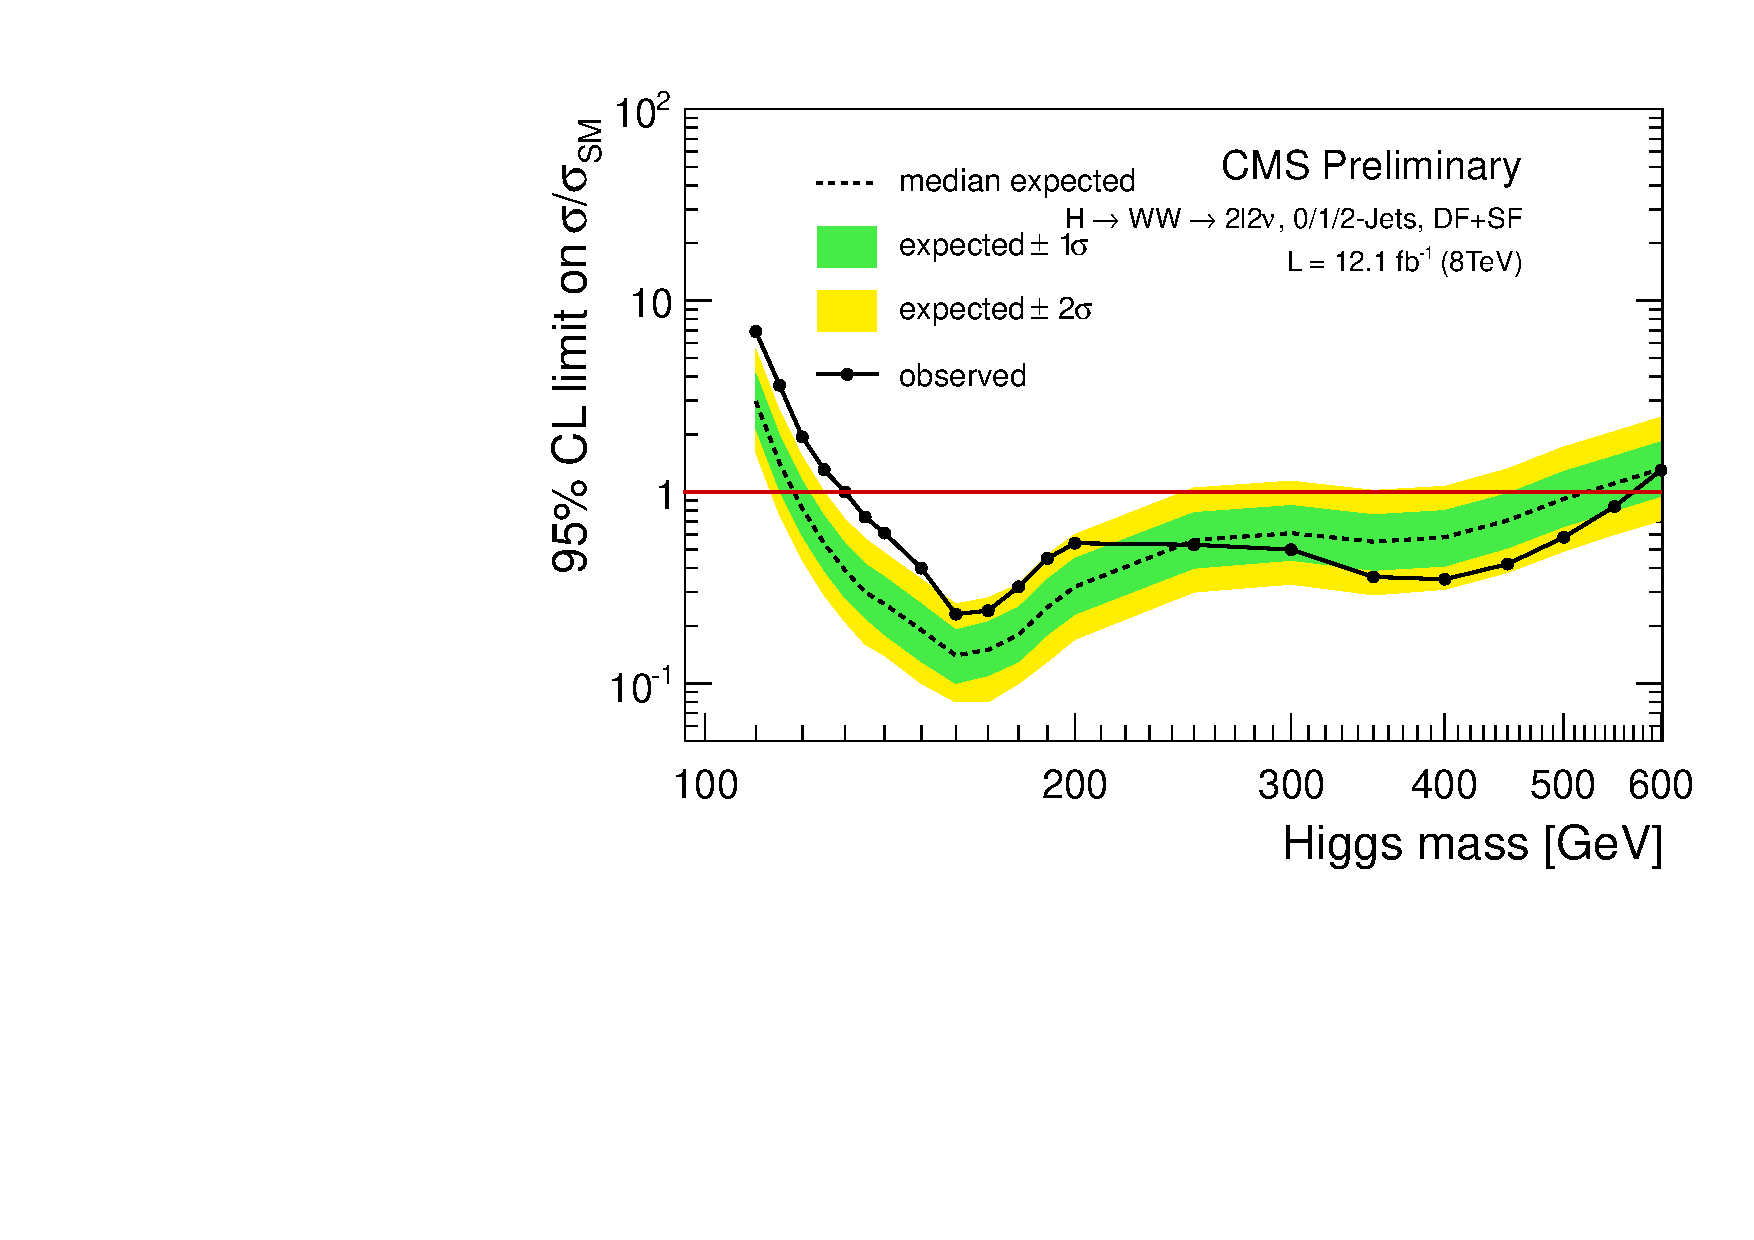
\includegraphics[width=.75\textwidth]{figures/table_limits_nj_shape2d_of_cut_sf_log.pdf}
\caption{Expected upper limits for SM Higgs in $\intlumiEightTeV$ at 8 TeV.
2D result is used for OF 0/1jet bin and cut-based result is used for VBF channel
and in the SF final states. }
\label{fig:uls_2d01_cut2_cutsf}
\end{figure}
% table
\begin{table}[!htbp]
\begin{center}
\begin{tabular}{c c c c c}
\hline
\vspace{-3mm} && \\
Higgs Mass & Observed  & Median expected & Expected range for 68\% & Expected range for 95\%   \\
\hline
110 & 6.89 & 2.97 & [2.14, 4.14] & [1.60, 5.55] \\
115 & 3.61 & 1.42 & [1.02, 1.98] & [0.76, 2.65] \\
120 & 1.94 & 0.82 & [0.59, 1.14] & [0.44, 1.53] \\
125 & 1.31 & 0.54 & [0.39, 0.75] & [0.29, 1.00] \\
130 & 1.00 & 0.39 & [0.28, 0.54] & [0.21, 0.72] \\
135 & 0.74 & 0.30 & [0.22, 0.42] & [0.16, 0.57] \\
140 & 0.61 & 0.26 & [0.18, 0.36] & [0.14, 0.48] \\
150 & 0.40 & 0.19 & [0.13, 0.26] & [0.10, 0.35] \\
160 & 0.23 & 0.14 & [0.10, 0.19] & [0.08, 0.26] \\
170 & 0.24 & 0.15 & [0.11, 0.21] & [0.08, 0.28] \\
180 & 0.32 & 0.18 & [0.13, 0.25] & [0.10, 0.33] \\
190 & 0.45 & 0.25 & [0.18, 0.35] & [0.13, 0.47] \\
200 & 0.54 & 0.32 & [0.23, 0.45] & [0.17, 0.60] \\
250 & 0.53 & 0.56 & [0.40, 0.78] & [0.30, 1.05] \\
300 & 0.50 & 0.61 & [0.44, 0.85] & [0.33, 1.14] \\
350 & 0.36 & 0.55 & [0.39, 0.76] & [0.29, 1.02] \\
400 & 0.35 & 0.58 & [0.41, 0.80] & [0.31, 1.07] \\
450 & 0.42 & 0.71 & [0.51, 0.98] & [0.38, 1.32] \\
500 & 0.58 & 0.92 & [0.66, 1.28] & [0.49, 1.72] \\
550 & 0.84 & 1.11 & [0.80, 1.54] & [0.60, 2.07] \\
600 & 1.30 & 1.32 & [0.95, 1.83] & [0.71, 2.46] \\
\vspace{-3mm} && \\
\hline
\end{tabular}
\caption{Expected upper limits for SM Higgs in $\intlumiEightTeV$ at 8 TeV.
2D result is used for OF 0/1jet bin and cut-based result is used for VBF channel
and in the SF final states. }
\label{tab:uls_2d01_cut2_cutsf}
\end{center}
\end{table}
%%%%%%%%%%


%%%%%%%%
\begin{table}[!htbp]
\begin{center}
\begin{tabular}{c | c c | c c  }
\hline \hline 
\vspace{-3mm} && \\
Higgs Mass(\GeV) & \multicolumn{2}{c}{cut-based} & \multicolumn{2}{c}{2D 0/1j DF+ cut-based} \\
\hline 
				 & Observed  & Expected 					 	& Observed  & Expected  \\
\hline \hline
115  & 2.2  & 1.1 & 3.0  & 1.5 \\    
125  & 1.7  & 2.4 & 2.8  & 3.7 \\
140  & 1.8  & 4.8 & 3.2  & 7.8 \\  
160  & 3.0  & 11.1 &  3.1  & 16.6 \\
200  & 2.0  & 4.4 &  1.6  & 6.1 \\
400  & 0.0  & 2.2 &  0.0  & 3.3 \\
600  & 0.0  & 1.2 &  0.0  & 1.5 \\   
\hline \hline
\end{tabular}
\caption{Expected and observed significances SM Higgs in $\intlumiEightTeV$ at 8 TeV. For cut-based, 
cut-based results in all channels are combined. For 2D, 2D results in DF 0/1jet bin results are 
combined with cut-based DF 2jet and SF 0/1/2jet results.}
\label{tab:significance_8TeV}
\end{center}
\end{table} 

%%%%%%%%%%%%%%%%%%%%%%%%%%%%%%




%%%%%%%%%%%
\clearpage 

\subsection{Final Results for the Higgs Search Combing 7 TeV and 8 TeV Data}
\label{sec:search_results_finalcomb}

In this section we document the Higgs search results combining the 7 \TeV\ and 8 \TeV\ data.  
For the 0 and 1 Jet bin final states, the 7 TeV analysis uses the shape based approach for all 
lepton flavor final states, while the 8 TeV analysis uses the cut-based approach for all 
final states or 2D based approach only in the $e\mu$ channel. 
The expected and observed limits with cut-based analysis in 8 TeV are shown in Figure~\ref{fig:uls_cut_comb} 
and Table~\ref{tab:uls_cut_comb}. 
The expected and observed limits with 2D analysis in 8 TeV are shown in Figure~\ref{fig:uls_2d01_cut2_cutsf_comb} 
and Table~\ref{tab:uls_2d01_cut2_cutsf_comb}. 
We also calculate the expected and observed significance in Table~\ref{tab:significance_7TeV8TeV}. 


%%%%%%%%%%%%%%%%%
% plot
\begin{figure}[!hbtp]
\centering
%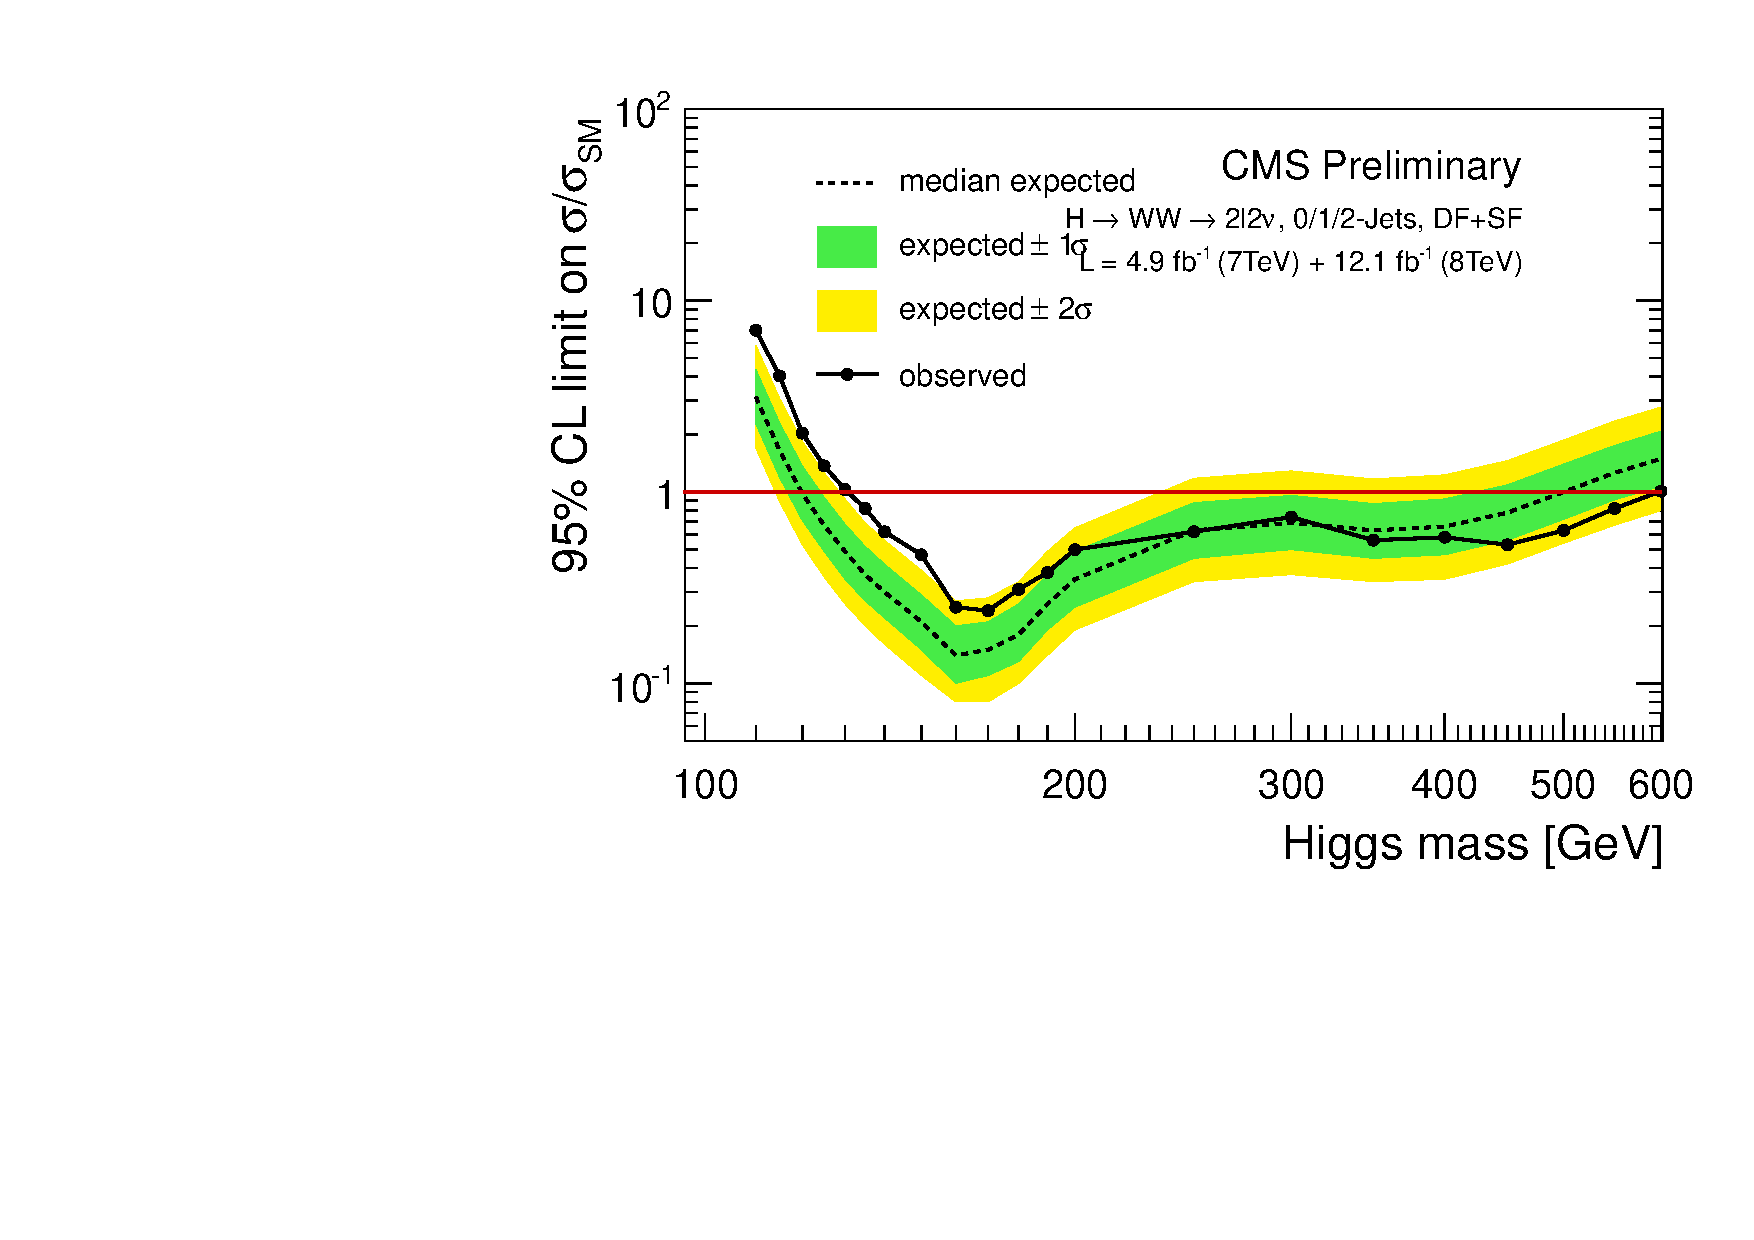
\includegraphics[width=.75\textwidth]{figures/table_limits_nj_8TeV_cut_7TeV_shape_log.pdf}
\caption{Expected and observed upper limits for SM Higgs combining the $\intlumiSevenTeV$ data
at 7 TeV and the $\intlumiEightTeV$ at 8 TeV.
For the 0 and 1 Jet bin final states, the 7 TeV analysis uses the shape based approach for all
lepton flavor final states, while the 8 TeV analysis uses cut-based approach in all final states.}
\label{fig:uls_cut_comb}
\end{figure}
% table
\begin{table}[!htbp]
\begin{center}
\begin{tabular}{c c c c c}
\hline
\vspace{-3mm} && \\
Higgs Mass & Observed  & Median expected & Expected range for 68\% & Expected range for 95\%   \\
\hline
110 & 7.00 & 3.14 & [2.26, 4.37] & [1.69, 5.86] \\
115 & 4.04 & 1.65 & [1.19, 2.30] & [0.89, 3.09] \\
120 & 2.03 & 0.98 & [0.71, 1.37] & [0.53, 1.84] \\
125 & 1.37 & 0.67 & [0.49, 0.94] & [0.36, 1.26] \\
130 & 1.03 & 0.49 & [0.35, 0.68] & [0.26, 0.92] \\
135 & 0.82 & 0.37 & [0.27, 0.52] & [0.20, 0.69] \\
140 & 0.62 & 0.30 & [0.22, 0.42] & [0.16, 0.56] \\
150 & 0.47 & 0.21 & [0.15, 0.29] & [0.11, 0.39] \\
160 & 0.25 & 0.14 & [0.10, 0.20] & [0.08, 0.27] \\
170 & 0.24 & 0.15 & [0.11, 0.21] & [0.08, 0.28] \\
180 & 0.31 & 0.18 & [0.13, 0.26] & [0.10, 0.34] \\
190 & 0.38 & 0.26 & [0.19, 0.37] & [0.14, 0.49] \\
200 & 0.50 & 0.35 & [0.25, 0.49] & [0.19, 0.65] \\
250 & 0.62 & 0.63 & [0.45, 0.88] & [0.34, 1.18] \\
300 & 0.74 & 0.69 & [0.50, 0.96] & [0.37, 1.29] \\
350 & 0.56 & 0.63 & [0.45, 0.87] & [0.34, 1.17] \\
400 & 0.58 & 0.66 & [0.47, 0.92] & [0.35, 1.23] \\
450 & 0.53 & 0.78 & [0.56, 1.09] & [0.42, 1.46] \\
500 & 0.63 & 1.00 & [0.72, 1.40] & [0.54, 1.87] \\
550 & 0.82 & 1.26 & [0.91, 1.75] & [0.67, 2.35] \\
600 & 1.01 & 1.49 & [1.07, 2.08] & [0.80, 2.78] \\
\vspace{-3mm} && \\
\hline
\end{tabular}
\caption{Expected and observed upper limits for SM Higgs combining the $\intlumiSevenTeV$ data
at 7 TeV and the $\intlumiEightTeV$ at 8 TeV.
For the 0 and 1 Jet bin final states, the 7 TeV analysis uses the shape based approach for all
lepton flavor final states, while the 8 TeV analysis uses cut-based approach in all final states.}
\label{tab:uls_cut_comb}
\end{center}
\end{table} 
%%%%%%%%%%

%%%%%%%%%%%%%%%%%
% plot
\begin{figure}[!hbtp]
\centering
%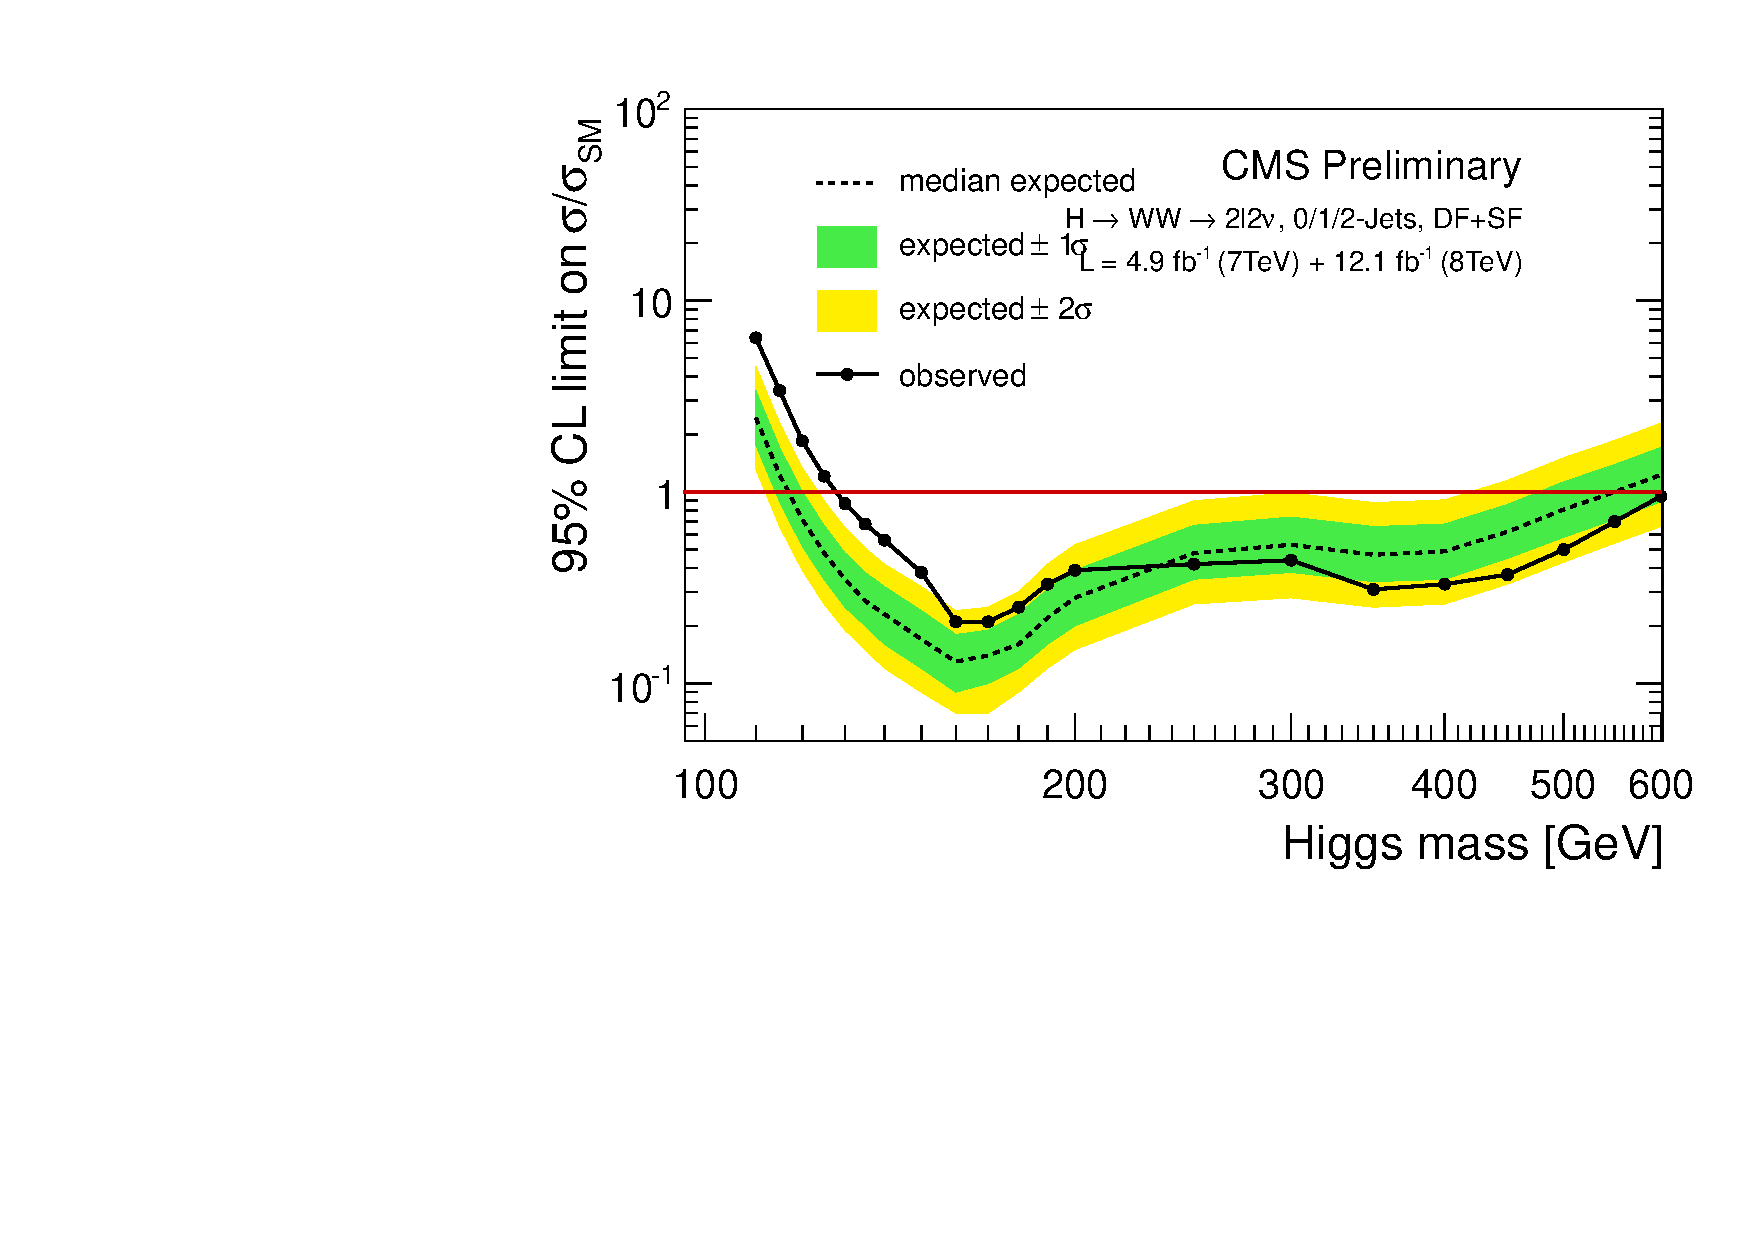
\includegraphics[width=.75\textwidth]{figures/table_limits_nj_8TeV_shape2d_of_cut_7TeV_shape_log.pdf}
\caption{Expected and observed upper limits for SM Higgs combining the $\intlumiSevenTeV$ data
at 7 TeV and the $\intlumiEightTeV$ at 8 TeV.
For the 0 and 1 Jet bin final states, the 7 TeV analysis uses the shape based approach for all
lepton flavor final states, while the 8 TeV analysis uses the 2D based approach 
in the $e\mu$ channel in 0/1jet bins and cut-based approch $e\mu$ 2jets and same flavor final states.}
\label{fig:uls_2d01_cut2_cutsf_comb}
\end{figure}
% table
\begin{table}[!htbp]
\begin{center}
\begin{tabular}{c c c c c}
\hline
\vspace{-3mm} && \\
Higgs Mass & Observed  & Median expected & Expected range for 68\% & Expected range for 95\%   \\
\hline 
\vspace{-3mm} && \\
110 & 6.39 & 2.44 & [1.76, 3.39] & [1.31, 4.55] \\
115 & 3.39 & 1.23 & [0.89, 1.71] & [0.66, 2.30] \\
120 & 1.85 & 0.72 & [0.52, 1.00] & [0.39, 1.34] \\
125 & 1.21 & 0.48 & [0.35, 0.67] & [0.26, 0.90] \\
130 & 0.87 & 0.35 & [0.25, 0.48] & [0.19, 0.65] \\
135 & 0.68 & 0.27 & [0.20, 0.38] & [0.15, 0.51] \\
140 & 0.56 & 0.23 & [0.16, 0.32] & [0.12, 0.42] \\
150 & 0.38 & 0.17 & [0.12, 0.24] & [0.09, 0.32] \\
160 & 0.21 & 0.13 & [0.09, 0.18] & [0.07, 0.24] \\
170 & 0.21 & 0.14 & [0.10, 0.19] & [0.07, 0.25] \\
180 & 0.25 & 0.16 & [0.12, 0.23] & [0.09, 0.30] \\
190 & 0.33 & 0.22 & [0.16, 0.31] & [0.12, 0.42] \\
200 & 0.39 & 0.28 & [0.20, 0.39] & [0.15, 0.53] \\
250 & 0.42 & 0.48 & [0.35, 0.67] & [0.26, 0.90] \\
300 & 0.44 & 0.53 & [0.38, 0.74] & [0.28, 0.99] \\
350 & 0.31 & 0.47 & [0.34, 0.66] & [0.25, 0.88] \\
400 & 0.33 & 0.49 & [0.35, 0.68] & [0.26, 0.91] \\
450 & 0.37 & 0.62 & [0.45, 0.86] & [0.33, 1.15] \\
500 & 0.50 & 0.81 & [0.58, 1.13] & [0.43, 1.51] \\
550 & 0.70 & 1.00 & [0.72, 1.39] & [0.54, 1.86] \\
600 & 0.95 & 1.23 & [0.89, 1.71] & [0.66, 2.29] \\
\hline
\end{tabular}
\caption{Expected and observed upper limits for SM Higgs combining the $\intlumiSevenTeV$ data
at 7 TeV and the $\intlumiEightTeV$ at 8 TeV.
For the 0 and 1 Jet bin final states, the 7 TeV analysis uses the shape based approach for all
lepton flavor final states, while the 8 TeV analysis uses the 2D based approach 
in the $e\mu$ channel in 0/1jet bins and cut-based approch $e\mu$ 2jets and same flavor final states.}
\label{tab:uls_2d01_cut2_cutsf_comb}
\end{center}
\end{table} 


\begin{table}[!htbp]
\begin{center}
\begin{tabular}{c | c c | c c  }
\hline \hline 
\vspace{-3mm} && \\
Higgs Mass(\GeV) & \multicolumn{2}{c}{cut-based in 8 TeV} & \multicolumn{2}{c}{2D in 0/1jet OF in 8 TeV} \\
\hline 
				 & Observed  & Expected 					 	& Observed  & Expected  \\
\hline \hline 
110 &  2.5 &   0.7 	& 2.8 	& 0.9 \\
115 &  2.8 &   1.3 	& 3.4 	& 1.6 \\ 
120 &  2.1 &   2.1 	& 2.8 	& 2.8 \\ 
125 &  2.1 &   3.0 	& 3.1 	& 4.1 \\ 
130 &  2.4 &   4.1 	& 3.1 	& 5.7 \\
140 &  2.4 &   6.3 	& 3.3 	& 9.0 \\
150 &  3.2 &   9.2 	& 3.7 	& 13.1 \\
160 &  3.4 &   14.7 & 3.5 	& 19.6 \\
170 &  2.8 &   13.0 & 2.9 	& 16.7 \\ 
180 &  2.2 &   9.9  & 2.1 	& 12.1 \\
190 &  1.3 &   7.0  & 1.5 	& 8.5 \\
200 &  1.1 &   5.5 	& 1.0 	& 6.8 \\
250 &  0.0 &   3.1 	& 0 	& 4.1 \\
300 &  0.1 &   2.9 	& 0 	& 3.8 \\
350 &  0.0 &   3.2 	& 0 	& 4.2 \\
400 &  0.0 &   3.1  & 0 	& 3.9 \\
450 &  0.0 &   2.6 	& 0 	& 3.1 \\
500 &  0.0 &   2.0 	& 0 	& 2.4 \\
550 &  0.0 &   1.7 	& 0 	& 2.0 \\   
600 &  0.0 &   1.4 	& 0	 	& 1.6 \\
\hline \hline
\end{tabular}
\caption{Expected and observed significances SM Higgs combining the $\intlumiSevenTeV$ data
at 7 TeV and the $\intlumiEightTeV$ at 8 TeV.  
For the 0 and 1 Jet bin final states, the 7 TeV analysis uses the shape based approach for 
all lepton flavor final states and cut-based approach is used for 2jet bin. For 8 TeV results, 
cut-based approach is used for all channels(left column). 2D approach is used for 
DF 0/1 jet channels and cut-based approach is used for all other channels(right column). 
}
\label{tab:significance_7TeV8TeV}
\end{center}
\end{table} 
